\subsection{Filtros paso bajo}
%%%%%%%%%%%%%%%%%%%%%%%%%%%%%%%%%%%%%
\begin{frame}\frametitle{Especificación de Filtros Paso Bajo}
  \vspace{-0.25cm}
  \begin{center}
      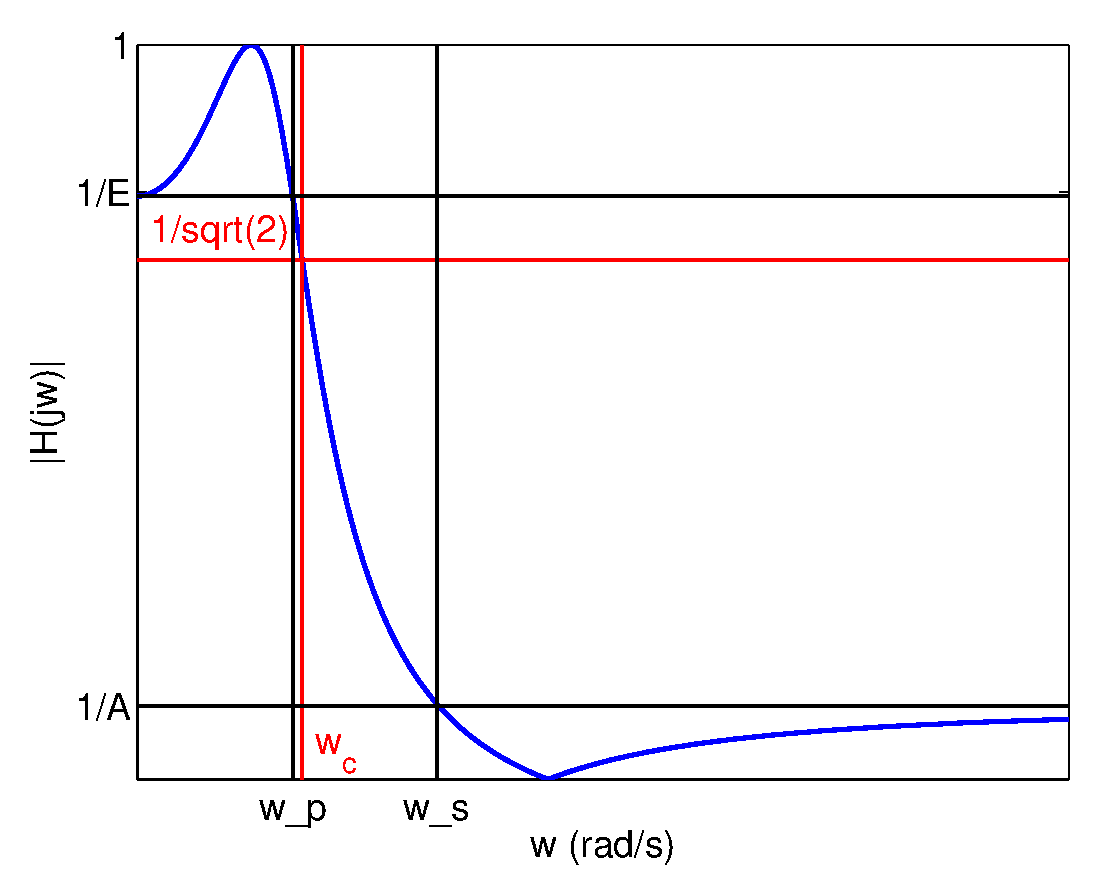
\includegraphics[width=4.8cm]{Figures/FiltroPB1_4}
  \end{center}
  \begin{alertblock}{Procedimiento de diseño}
      \begin{itemize}\small\vspace{0.05cm}
          \item Filtros paso bajo continuos con $|H(j\omega)|=\frac{1}{1+P(\omega)}$\vspace{0.05cm}
          \item $P(\omega)$ se determina de forma que $|H(j\omega)|$ se aproxime al filtro ideal\vspace{0.05cm}
          \item Para otros tipos de filtros, utilizamos transformaciones espectrales\vspace{0.05cm}
      \end{itemize}
  \end{alertblock}
\end{frame}


\begin{frame}\frametitle{Especificación de Filtros Paso Bajo}
  \begin{columns}[T]
    \begin{column}{7cm}
      \footnotesize
      \vspace{0.6cm}
          \begin{itemize}
            \scriptsize
            \item Frecuencia corte $\color{blue}\omega_c: |H(j\omega_c)|=\frac{1}{\sqrt{2}}$  (3 dB)
            \item Banda de paso: $\color{blue}[0,\omega_p]$\\
            Frecuencia paso: $\color{blue}\omega_p$\\
            Atenuación máxima banda paso (dB):
            \hspace{1cm}$\color{blue}\alpha_p=-20 \log_{10}(\frac{1}{E})$, $\color{blue}\:\:E=\sqrt{1+\epsilon^2}$
          \\
          Rizo banda paso: $\delta_p$
              \item Banda de transición: $\color{blue}[\omega_p,\omega_s]$
              \vspace{-0.1cm}
              \item Banda de supresión: $\color{blue}[\omega_s,\infty]$\\
              Frecuencia supresión: $\color{blue}\omega_s$\\
              Atenuación mínima banda supresora (dB):
              \hspace{1cm}$\color{blue}\alpha_s=-20 \log_{10}(\frac{1}{A})$\\
              \vspace{0.1cm}
              Rizo banda supresora: $\color{blue}\delta_s$
              \item Razón de transición, p. selectividad: $\color{blue}k=\frac{\omega_p}{\omega_s}$
              \item Parámetro de discriminación: $\color{blue}k_1=\frac{\epsilon}{\sqrt{A^2-1}}$
          \end{itemize}
      \end{column}
      \begin{column}{6cm}
          \footnotesize
          \hspace{1.5cm}Filtro ideal\\
          \hspace{2.1cm}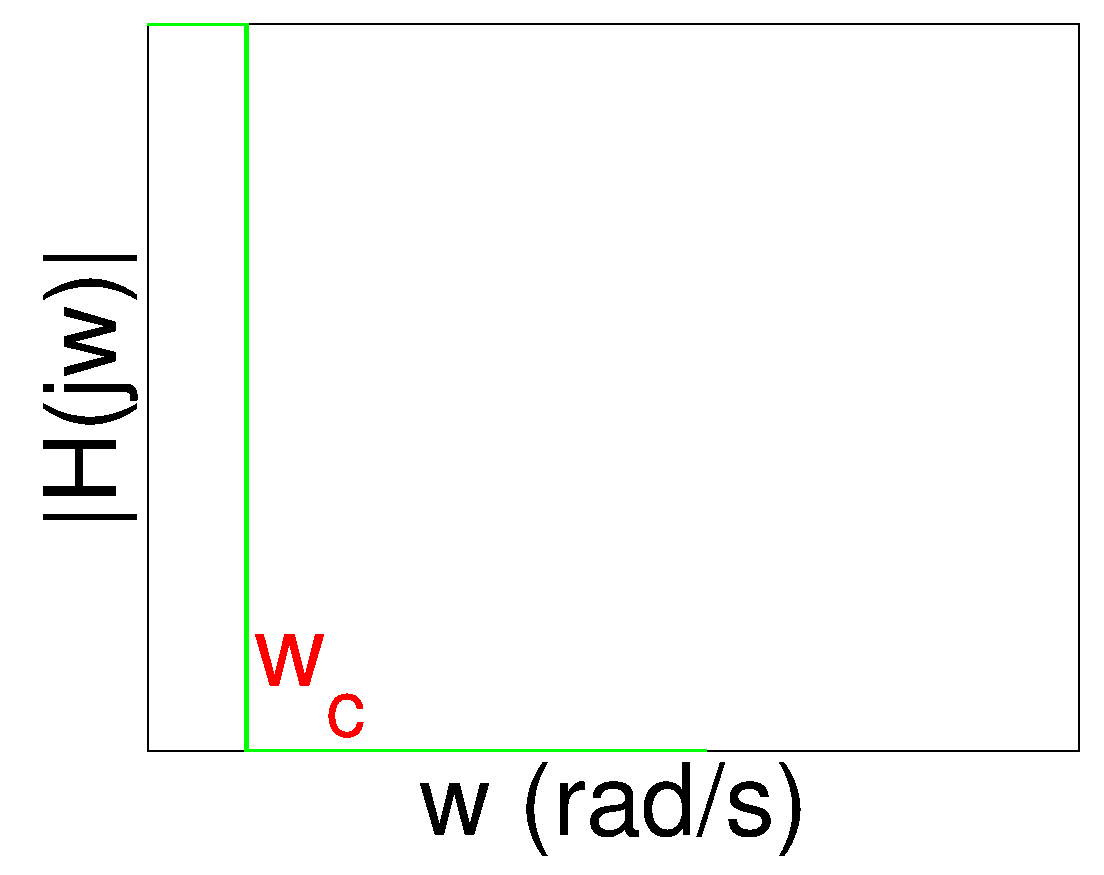
\includegraphics[width=4cm]{Figures/FiltroPB0_2}
          \hspace{3cm}Filtro real\\
          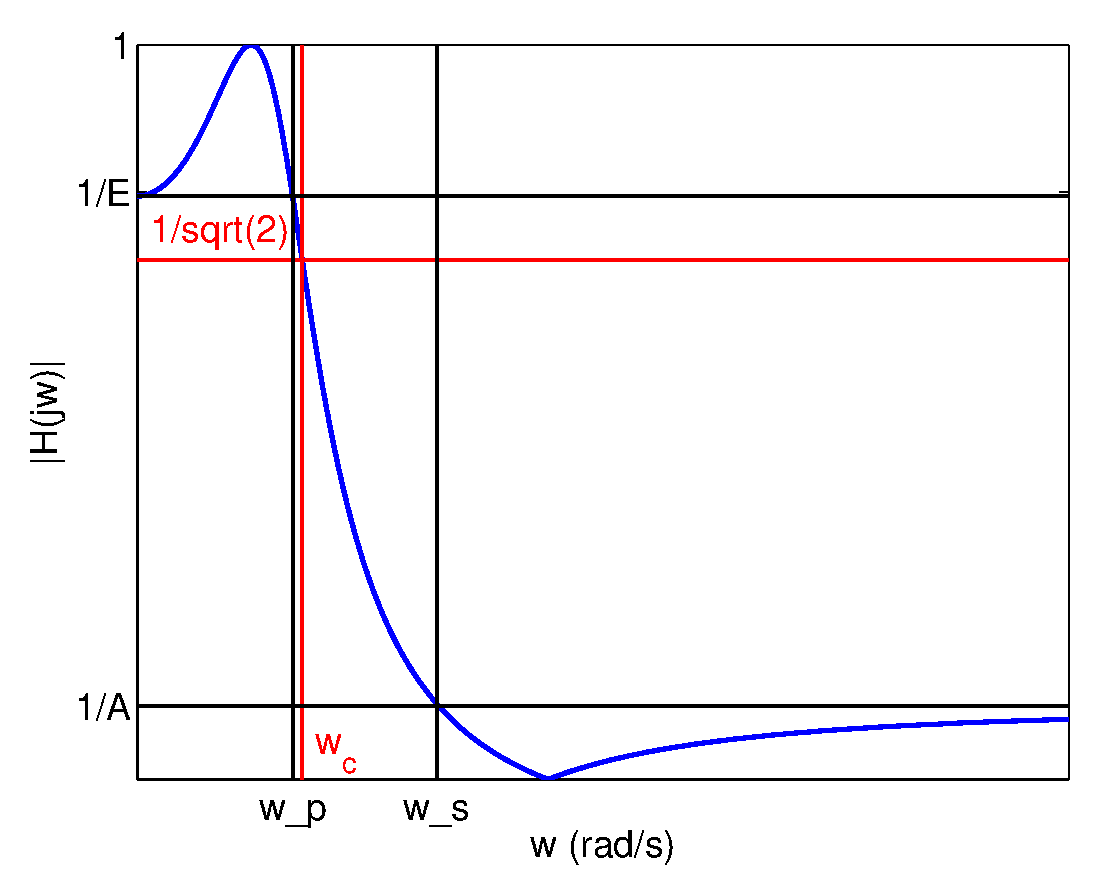
\includegraphics[width=4cm]{Figures/FiltroPB1_4}
      \end{column}
  \end{columns}
\end{frame}

\begin{frame}\frametitle{Especificación de Filtros Paso Bajo}
  \vspace{-0.9cm}
  \begin{center}
      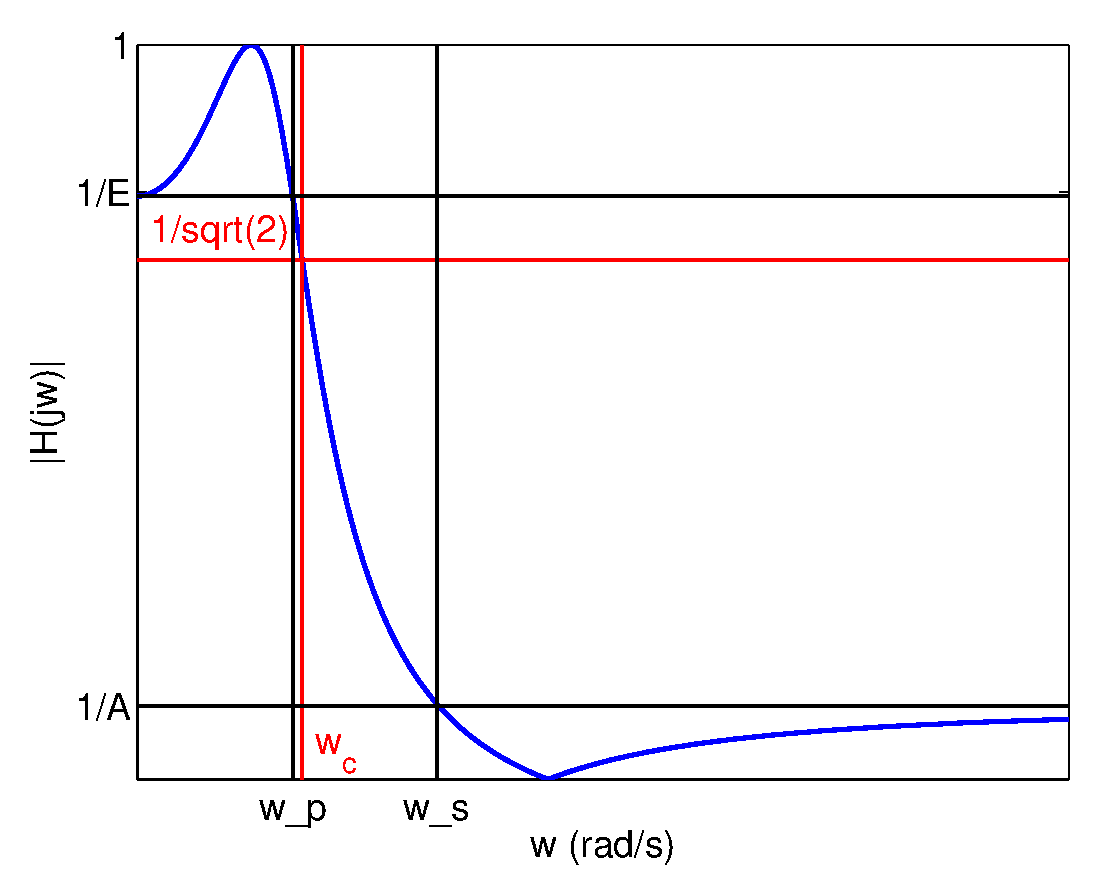
\includegraphics[width=4.8cm]{Figures/FiltroPB1_4}
  \end{center}
  \begin{alertblock}{Parámetros a especificar en un filtro paso bajo}
      \begin{itemize}
          \item $\omega_p$: Frecuencia de paso (rad/s o Hz)
          \item $\omega_s$: Frecuencia de supresión (rad/s o Hz)
          \item $\alpha_p$: Atenuación máxima en la banda de paso (dB)
          \item $\alpha_s$: Atenuación mínima en la banda de supresión (dB)
      \end{itemize}
  \end{alertblock}
\end{frame}

\begin{frame}\frametitle{Algunos tipos de filtros paso bajo}
  \begin{columns}[T]
      \hspace{-0.2cm}\begin{column}{4cm}
          \scriptsize
          \visible<2->{
              \hspace{1.5cm}Butterworth
              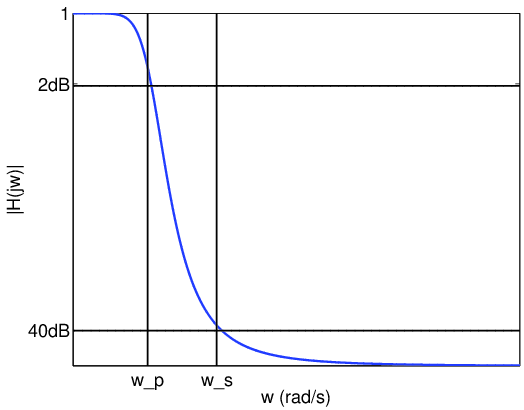
\includegraphics[width=4cm]{Figures/FiltroPB2_Butter.png}
          }
          \visible<4->{
              \hspace{1.5cm}Chebyshev I
              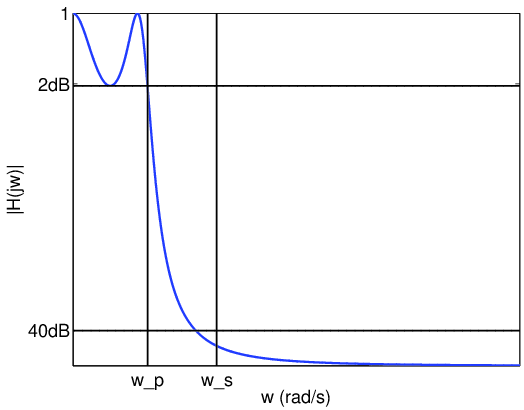
\includegraphics[width=4cm]{Figures/FiltroPB2_Cheby1.png}
          }
      \end{column}
      \hspace{-0.2cm}\begin{column}{4cm}
          \scriptsize
          \visible<2->{
              \hspace{1.9cm}Eliptico
              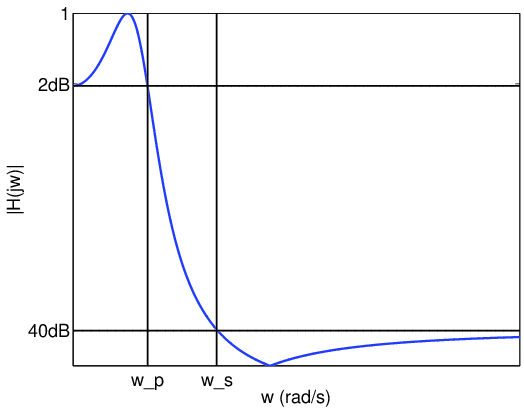
\includegraphics[width=4cm]{Figures/FiltroPB2_Ellip.png}
          }
          \visible<4->{
              \hspace{1.4cm}Chebyshev II
              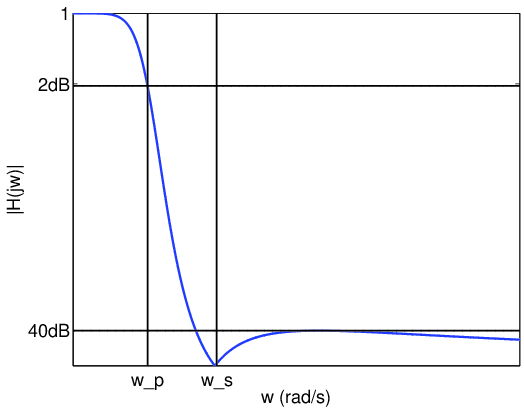
\includegraphics[width=4cm]{Figures/FiltroPB2_Cheby2.png}
          }
          \footnotesize
      \end{column}
      \hspace{-0.3cm}\begin{column}{4.6cm}
      \footnotesize
      \visible<3->{
          \hspace{0.3cm} Diferencias:
          \vspace{-0.1cm}
          \begin{itemize}
              \item Rizado:\\
              {\scriptsize
                  \color{blue}$\star$ Butterworth\color{black}:\\ \hspace{0.5cm} Sin rizado\\
                  \color{blue}$\star$ Elíptico\color{black}:\\ \hspace{0.5cm} Dos bandas\\
              }
          \scriptsize
      }
      \visible<4->{
          \color{blue}$\star$ Chebyshev I\color{black}: \\ \hspace{0.5cm}Banda paso\\
          \color{blue}$\star$ Chebyshev II\color{black}: \\\hspace{0.5cm}Banda supresión
      }

      \visible<5->{

          \item Función Transferencia:

          {\scriptsize
          \color{blue}$\star$ \color{black} Posición de los polos/ceros\\
          \color{blue}$\star$ \color{black} Orden (\# polos)\\
          \visible<6->{
              \color{blue}$\star$ \color{black} Banda de transición (para un mismo orden):\\
              \hspace{0.2cm} \color{blue}Butterworth\color{black}:\\ \hspace{0.5cm}caída lenta\\
              \hspace{0.2cm} \color{blue}Eliptico\color{black}:\\ \hspace{0.5cm}caída rápida\\
              \hspace{0.2cm} \color{blue}Chebyshev I\color{black}: \\ \hspace{0.5cm} caída rápida paso\\
              \hspace{0.2cm} \color{blue}Chebyshev II\color{black}:\\ \hspace{0.5cm} caída rápida supresión\\
          }
      }
  }

  \end{itemize}
  \end{column}

\end{columns}


\end{frame}


%%%%%%%%%%%%%%%%%%%%%%%%%%%%%%%%

\begin{frame}
\frametitle{Filtro de Butterworth}

\begin{columns}[T]
\hspace{-0.5cm}\begin{column}{8cm}

\footnotesize


\alert{\hspace{0.3cm}$\displaystyle |H(j\omega)|^2=\frac{1}{1+\left (\frac{\omega}{\omega_c}\right )^{2N}}$}

\visible<2->{

\hspace{0.3cm}\alert{$\displaystyle  H(s)=\frac{\omega_c^N}{\prod_{l=1}^N (s-p_l)}$}, con \alert{$\displaystyle p_l=\omega_c e^{\frac{j\pi(N+2l-1)}{2N}}$}}

\vspace{0.1cm}


\vspace{-0.1cm}

\visible<4->{
\begin{itemize}
\item Para una $\omega_c$ fija,
si aumenta $N$ disminuye ancho banda de transición.

\visible<5->{
\item Dados unos valores $\omega_p$, $\omega_s$, $\alpha_p$, $\alpha_s$, determinar el filtro de menor $N$ que los cumple (fijando $\omega_c$).
}

\color{gray}

\scriptsize

\visible<6->{
  $\!\!\!\!\left . \begin{array}{l}
\alpha_p=-20 log_{10} \frac{1}{E} \\ \alpha_s=-20 log_{10} \frac{1}{A}\end{array}\right \}$ }   \visible<7->{ $\rightarrow \displaystyle\left . \begin{array}{l}
E= 10^{\frac{ \alpha_p}{20}} \\ A=10^{\frac{ \alpha_s}{20}} \end{array}\right \}$}

\end{itemize}
}

\end{column}
\hspace{-0.3cm}\begin{column}{4cm}
\visible<1->{
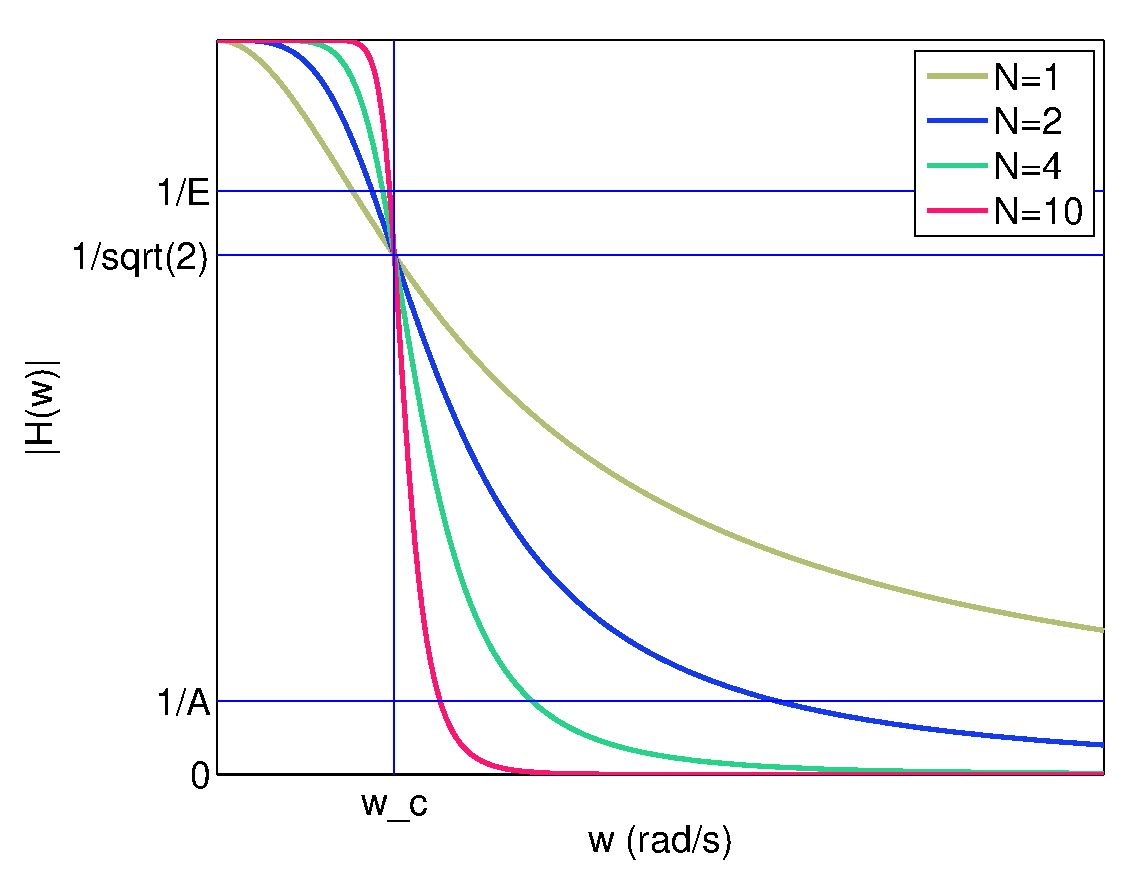
\includegraphics[width=3.5cm]{Figures/FiltroPB_Butter}
}

\vspace{0.1cm}

\visible<3->{
\hspace{0.8cm}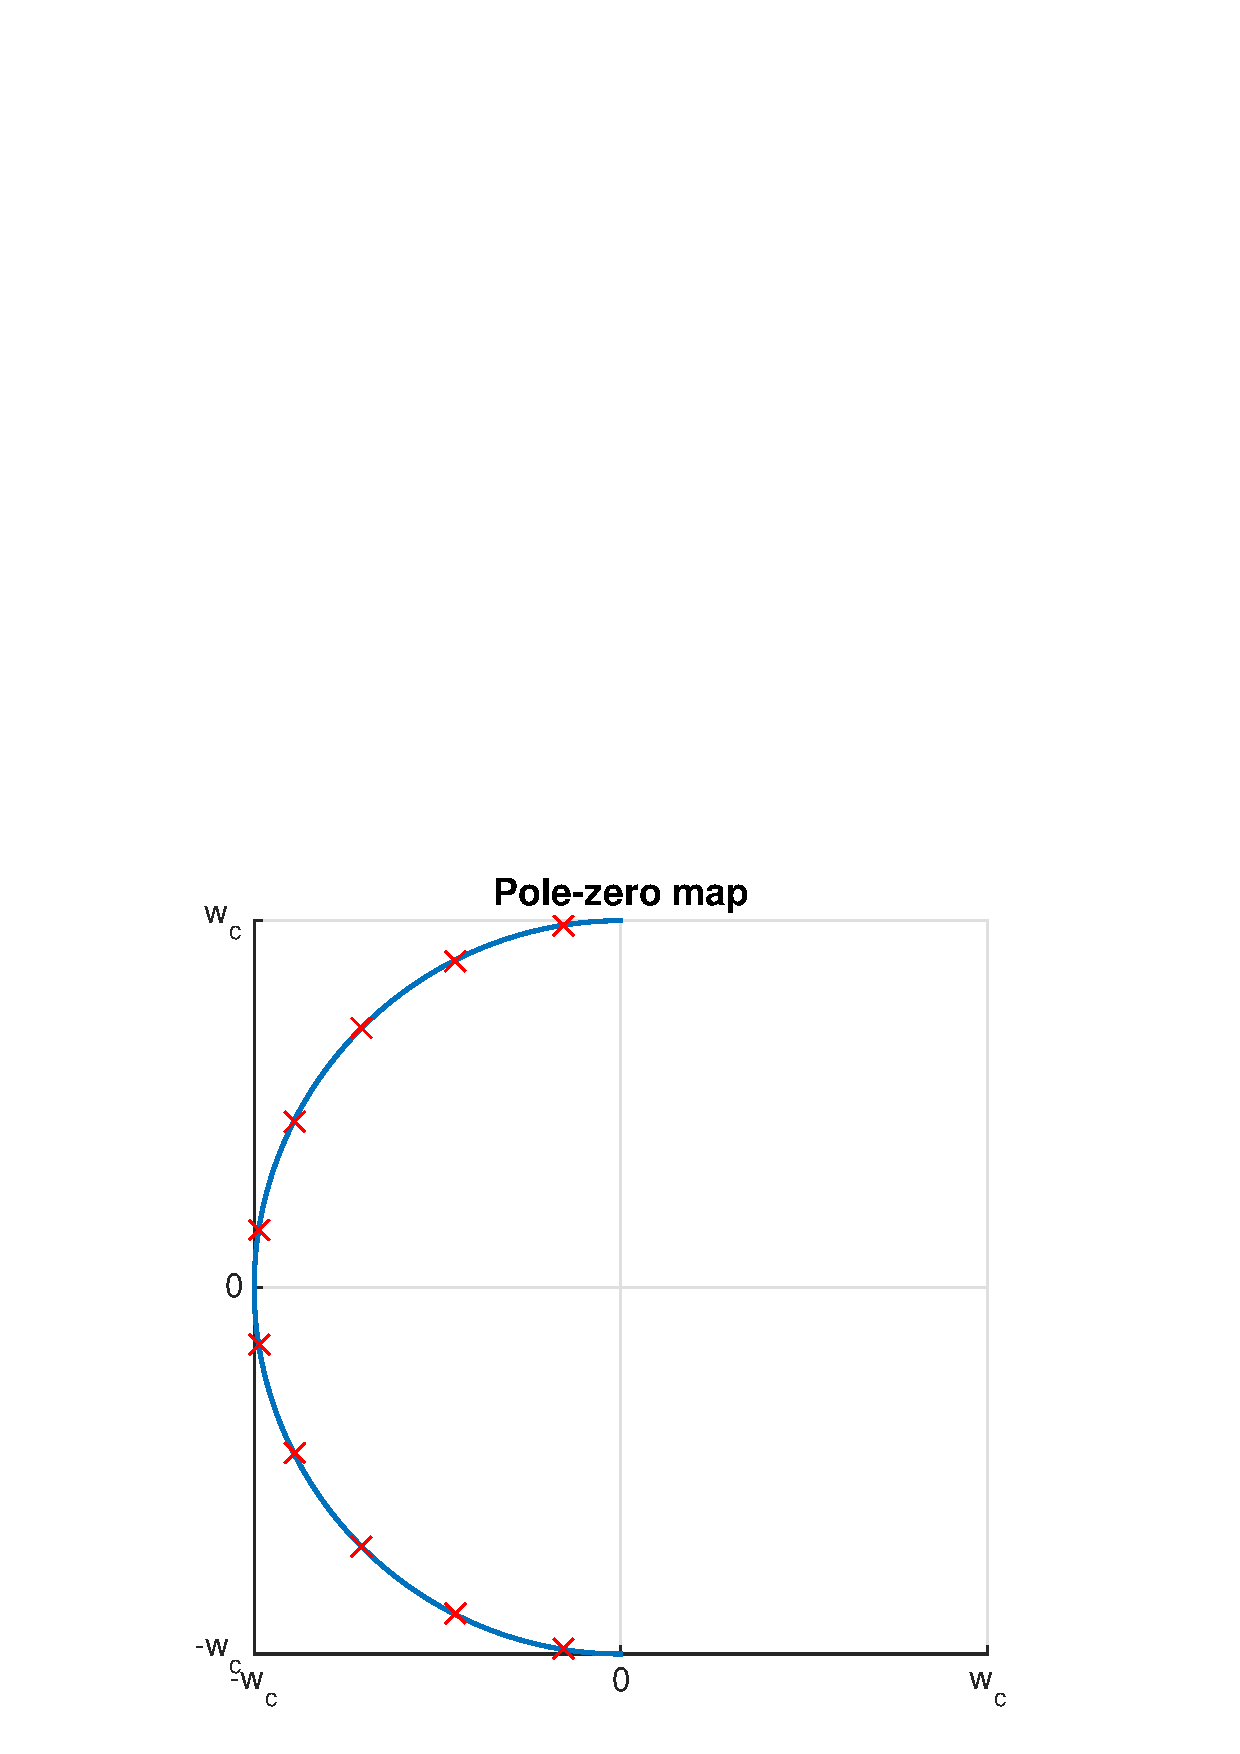
\includegraphics[width=2.2cm]{Figures/PolesButter}
}

\end{column}
\end{columns}

\vspace{-0.1cm}



{

\scriptsize
\color{gray}


\visible<6->{
\hspace{0.0cm} $\!\!\!\!\left . \begin{array}{l}|H(j\omega_p)|^2=\frac{1}{1+\left (\frac{\omega_p}{\omega_c}\right )^{2N}}=\frac{1}{E^2} \\
|H(j\omega_s)|^2=\frac{1}{1+\left (\frac{\omega_s}{\omega_c}\right )^{2N}}=\frac{1}{A^2}\\
\end{array}\right \}  $}   \visible<8->{$\rightarrow \!\!\left . \begin{array}{l}E^2-1=\left (\frac{\omega_p}{\omega_c}\right )^{2N} \\
A^2-1=\left (\frac{\omega_s}{\omega_c}\right )^{2N} \\
\end{array}\right \}\rightarrow $ $ \frac{A^2-1}{E^2-1}=\left (\frac{\omega_s}{\omega_p}\right )^{2N} \rightarrow $

\vspace{-.1cm}
\hspace{0.0cm}   $log_{10} \frac{A^2-1}{E^2-1}=2N log_{10}\frac{\omega_s}{\omega_p}\rightarrow$ $\alert{N=\frac{1}{2}\frac{log_{10} \frac{A^2-1}{E^2-1}}{log_{10}\frac{\omega_s}{\omega_p}}} \rightarrow$  $N=\frac{log_{10} \frac{1}{k_1}}{log_{10}\frac{1}{k}} $
}

\visible<9>{
\hspace{0.0cm}  $A^2-1=\left (\frac{\omega_s}{\omega_c}\right )^{2N}\rightarrow$  $\omega_c^{2N}=\frac{\omega_s^{2N}}{A^2-1} \rightarrow$     \alert{$\omega_c=\frac{\omega_s}{(A^2-1)^{\frac{1}{2N}}}$}
}

}

\end{frame}


%%%%%%%%%%%%%%%%%%%%%%%%%%%%%%%

\begin{frame}
\frametitle{Filtro de Butterworth (ejemplo)}

\begin{itemize}

{
\scriptsize
\item \color{olivegreen} Determinar el filtro de Butterworth de orden más bajo con una atenuación en la banda de paso máxima de 1dB a 1KHz y una atenuación mínima en la banda de supresión de 40dB a 5KHz.

\begin{columns}[T]
\hspace{0.8cm}\begin{column}{7.1cm}
\color{gray}

\visible<2->{

 $\begin{array}{l}\!\!\!\left .\begin{array}{l}\omega_p=2\pi*1000\\
 \omega_s=2\pi*5000\\
 \alpha_p=1dB\\
 \alpha_s=40\end{array}\!\!\!\right \} \rightarrow\\ \: \\ \: \end{array}$ } \visible<3->{$\!\!\!\!\!\!\begin{array}{l}E= 10^{\frac{ \alpha_p}{20}}=1.122 \\ A=10^{\frac{ \alpha_s}{20}}=100\\
 N\!=\!\frac{1}{2}\frac{log_{10} \frac{A^2-1}{E^2-1}}{log_{10}\frac{\omega_s}{\omega_p}} \!=\!3.28 \rightarrow 4 \\
 \omega_c=\frac{\omega_s}{(A^2-1)^{\frac{1}{2N}}}\approx 9935 \end{array}$}
 \end{column}
\hspace{-1cm} \begin{column}{4cm}
\vspace{-0.2cm}
\visible<4->{ 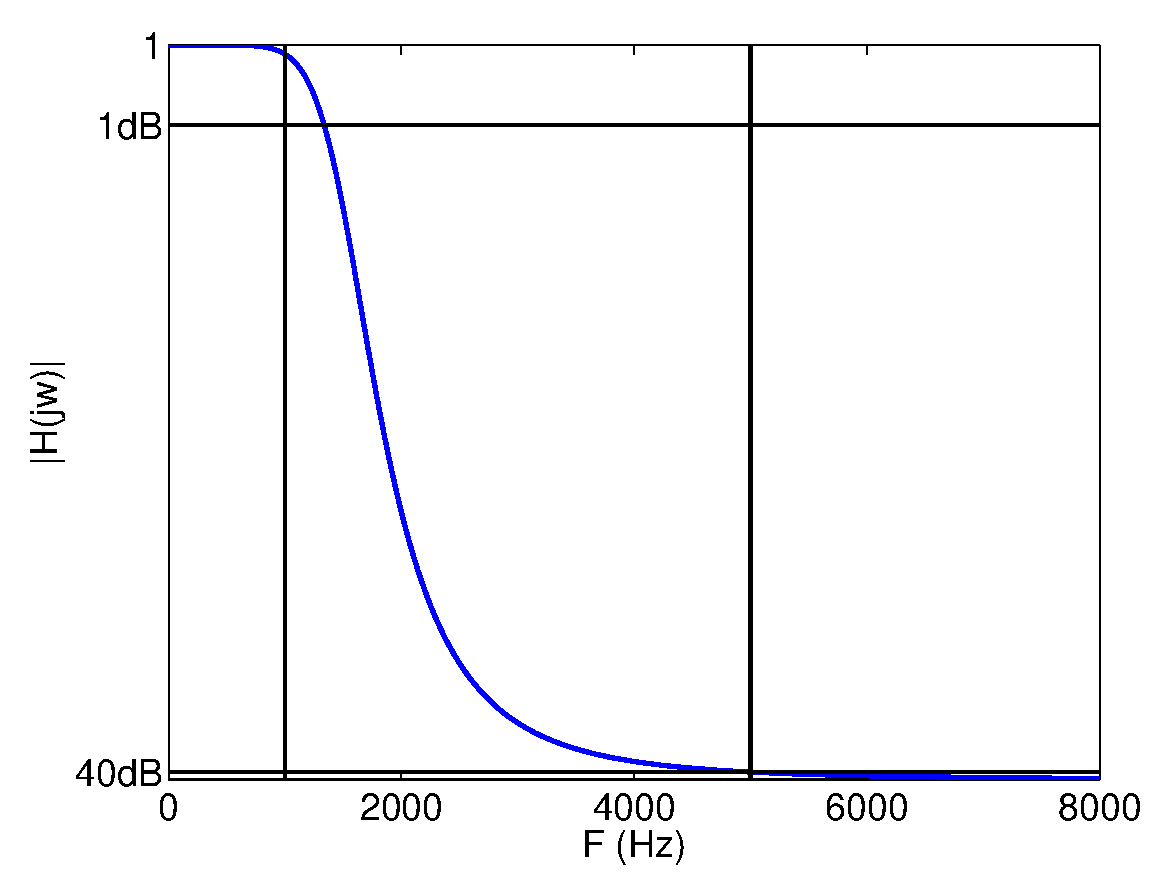
\includegraphics[width=4cm]{./Figures/FiltroPB_ButterEx.eps}}
 \end{column}
 \end{columns}

}
\visible<5->{
{

\vspace{-0.5cm}

\footnotesize
\item Con Matlab:

\begin{itemize}
\item \alert{\texttt{[N,wc]=buttord(wp,ws,ap,as,'s')}}
\begin{itemize}
\color{gray}
\item Calcula el orden \texttt{N} del filtro y la frecuencia de corte \texttt{wc}.
\item \texttt{wp}, \texttt{ws} en rad/s.
\item \texttt{ap}, \texttt{as} en dB.
\item 's' para que calcule los valores del filtro de continuo.
\end{itemize}
\item \alert{\texttt{[B,A]=butter(N,wc,'low','s')}}
\begin{itemize}
\color{gray}
\item Calcula el numerador y denominador de $H(s)$.
\end{itemize}
\item \alert{\texttt{[Hw,w]=freqs(B,A)}}
\begin{itemize}
\color{gray}
\item Calcula la $H(j\omega)$ del filtro para las frecuencias \texttt{w}.
\end{itemize}

\end{itemize}
}
}
\end{itemize}

\end{frame}

%%%%%%%%%%%%%%%%%%%%%%%%%%%%%%%%%%%%%%

\begin{frame}
\frametitle{Filtro de Chebyshev Tipo I}

\begin{columns}[T]
\hspace{0.4cm}\begin{column}{8cm}

\footnotesize

\footnotesize


\hspace{0.4cm}\alert{$\displaystyle |H(j\omega)|^2=\frac{1}{1+\epsilon^2 T_N^2(\omega/\omega_p)}$}

\vspace{0.1cm}

\hspace{0.4cm}$T_N(w)=\left \{ \begin{array}{l}cos(N \cdot acos(\omega)) \:\:\:\:\:\:\:\: |\omega|\le 1\\ cosh(N \cdot acosh(\omega)) \:\:\: |\omega|> 1\end{array} \right .$

\visible<2->{

\hspace{0.4cm}\alert{$\displaystyle  H(s)=\frac{K_N}{\prod_{l=1}^N (s-p_l)}$}, con \alert{$\displaystyle p_l=\sigma_l+j\omega_l$}

\vspace{0.1cm}

\hspace{0.4cm}$\sigma_l=-\omega_p \frac{\gamma^2-1}{2\gamma}sin\left( \frac{(2l-1)\pi}{2N}\right)$, \hspace{0.5cm}$\gamma=\left ( \frac{1+\sqrt{1+\epsilon^2}}{\epsilon} \right )^{\frac{1}{N}}$

\vspace{0.1cm}

\hspace{0.4cm}$\omega_l= \omega_p \frac{\gamma^2+1}{2\gamma}cos\left( \frac{(2l-1)\pi}{2N}\right)$, \hspace{0.5cm}$E=\sqrt{1+\epsilon^2}$}


\vspace{-0.1cm}

\begin{itemize}

\visible<4->{

\item Para una $\omega_p$ fija,
si aumenta $N$ disminuye ancho de la banda de transición.


}
\end{itemize}




\end{column}
\hspace{-0.5cm}\begin{column}{4cm}
\visible<1->{
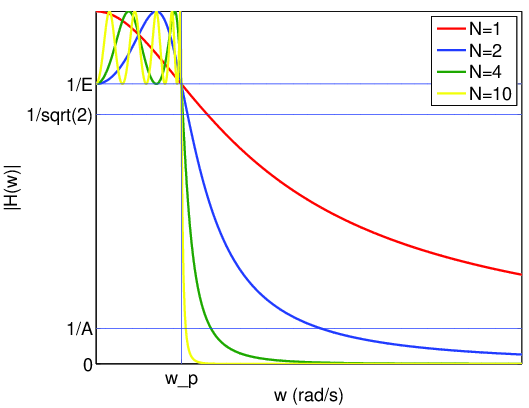
\includegraphics[width=3.5cm]{Figures/FiltroPB_Cheby1.png}
}

\vspace{0.1cm}


\visible<3->{
\hspace{0.8cm}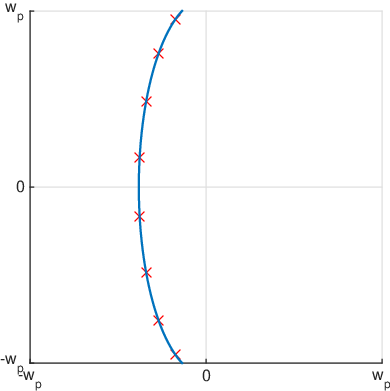
\includegraphics[width=2.2cm]{Figures/PolesCheby1.png}
}

\end{column}
\end{columns}

\vspace{0.1cm}

\footnotesize
\begin{itemize}



\visible<5->{
\item Determinar el filtro de menor $N$ para valores dados de  $\omega_p$, $\omega_s$, $\alpha_p$, $\alpha_s$.
}
\vspace{0.1cm}
{

\color{gray}

\scriptsize

  $\!\!\!\!\left . \begin{array}{l}
\alpha_p=-20 log_{10} \frac{1}{E} \\ \alpha_s=-20 log_{10} \frac{1}{A}\end{array}\right \}$ }   \visible<7->{ $\rightarrow \displaystyle\left . \begin{array}{l}
E= 10^{\frac{ \alpha_p}{20}} \\ A=10^{\frac{ \alpha_s}{20}} \end{array}\right \}$ $\rightarrow \epsilon=\sqrt{E^2-1}$ }

\vspace{-0.3cm}

\visible<6->{
$
|H(j\omega_s)|^2=\frac{1}{1+\epsilon^2 cosh^2( N\cdot acosh(\omega_s/\omega_p))}=\frac{1}{A^2} \rightarrow$}   \visible<8->{\alert{$
N=\frac{acosh \left ( \frac{\sqrt{A^2-1}}{\epsilon} \right)}{acosh(\omega_s/\omega_p)} $} $\rightarrow N=\frac{acosh \frac{1}{k_1}}{acosh\frac{1}{k}} $
}


\end{itemize}
\end{frame}

%%%%%%%%%%%%%%%%%%%%%%%%%%%%%%%

\begin{frame}
  \frametitle{Filtro de Chebyshev Tipo I (ejemplo)}
  
  \begin{itemize}
    
    \scriptsize
    \item \color{olivegreen} Determinar el filtro de Chebyshev tipo I de orden más bajo con una atenuación en la banda de paso máxima de 1dB a 1KHz y una atenuación mínima en la banda de supresión de 40dB a 5KHz.
    
    \begin{columns}[T]
      \hspace{0.7cm}\begin{column}{7.1cm}
      \color{gray}
      {$\begin{array}{l}\!\!\!\left .\begin{array}{l}
        \omega_p=2\pi\cdot 1000\\
        \omega_s=2\pi\cdot 5000\\
        \alpha_p=1dB\\
        \alpha_s=40\end{array}\!\!\!\right \} \rightarrow\\ \: \\ \: \end{array}$ } \visible<2->{$\!\!\!\!\!\!\begin{array}{l}E= 10^{\frac{ \alpha_p}{20}}=1.122 \\ A=10^{\frac{ \alpha_s}{20}}=100\\ \epsilon=\sqrt{E^2-1}=0.5088 \\
        N\!=\!\frac{acosh \!\left (\! \frac{\sqrt{A^2-1}}{\epsilon}\! \right)}{acosh(\omega_s/\omega_p)} \!=\!2.61 \rightarrow 3 \end{array}$}
      \end{column}
      \hspace{-0.9cm} \begin{column}{4cm}
        \vspace{-0.2cm}
        \visible<3->{ 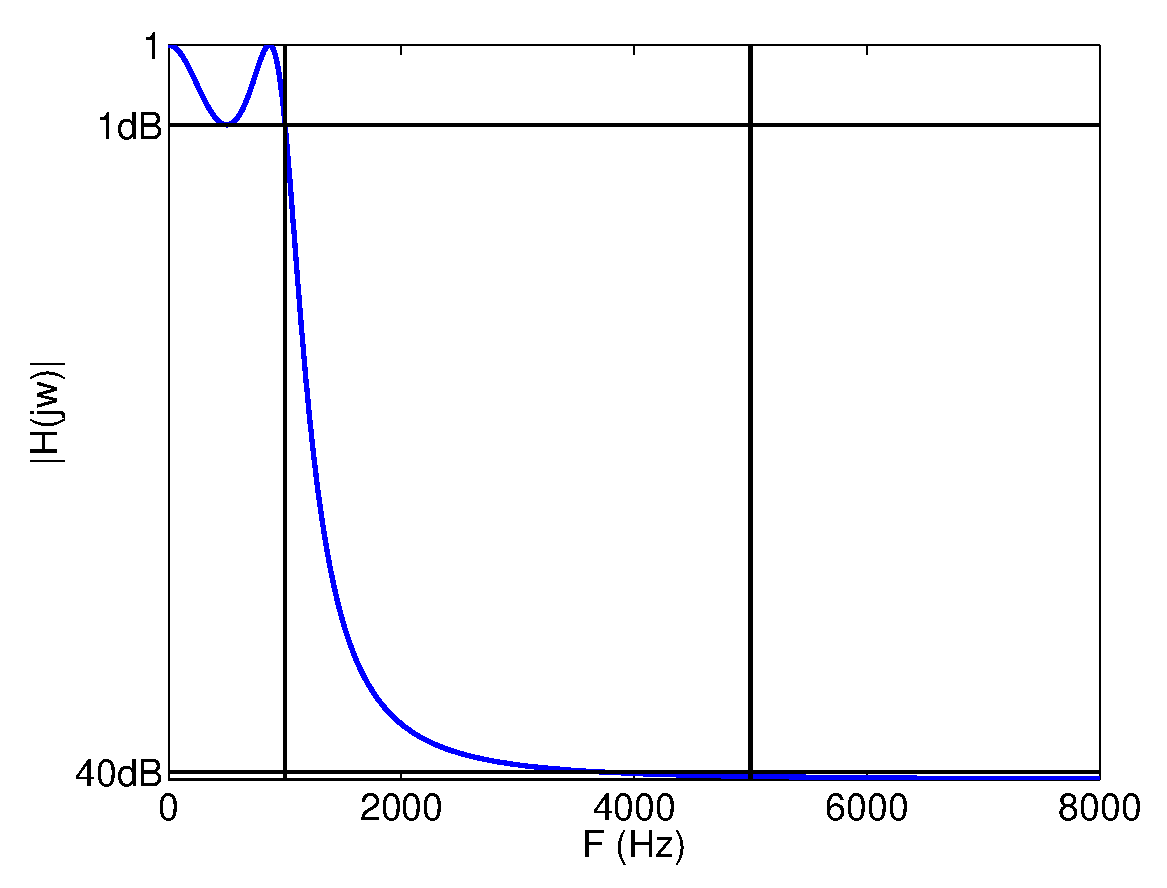
\includegraphics[width=4cm]{./Figures/FiltroPB_Cheby1Ex.eps}}
      \end{column}
    \end{columns}
  
    \vspace{-0.5cm}
    
    \footnotesize
    \item Con Matlab:
    
    \begin{itemize}
      \item \alert{\texttt{[N,wc]=cheb1ord(wp,ws,ap,as,'s')}}
      \begin{itemize}
        \color{gray}
        \item Calcula el orden \texttt{N} del filtro y la frecuencia de corte \texttt{wc}.
        \item \texttt{wp}, \texttt{ws} en rad/s.
        \item \texttt{ap}, \texttt{as} en dB.
        \item 's' para que calcule los valores del filtro de continuo.
      \end{itemize}
      \item \alert{\texttt{[B,A]=cheby1(N,ap,wc,'low','s')}}
      \begin{itemize}
        \color{gray}
        \item Calcula el numerador \texttt{B} y denominador \texttt{A} de $H(s)$
      \end{itemize}
      \item \alert{\texttt{[Hw,w]=freqs(B,A)}}
      \begin{itemize}
        \color{gray}
        \item Calcula la $H(j\omega)$ del filtro, \texttt{Hw}, para las frecuencias \texttt{w}
      \end{itemize}
        
    \end{itemize}
    
  \end{itemize}
\end{frame}
  
  
  %%%%%%%%%%%%%%%%%%%%%%%%%%%%%%%%%%%%
  
  
  \begin{frame}
  \frametitle{Filtro de Chebyshev Tipo II}
  
   \vspace{-0.2cm}
  
  \begin{columns}[T]
  \hspace{0.3cm}\begin{column}{8cm}
  
  \footnotesize
  
  \visible<1->{
  
  \hspace{0.4cm}\alert{$\displaystyle |H(jw)|^2=\frac{1}{1+\epsilon^2 \frac{T_N^2(\omega_s/\omega_p)}{T_N^2(\omega_s/w)}}$}
  
  \hspace{0.4cm}$T_N(w)=\left \{ \begin{array}{l}cos(N \cdot acos(w)) \:\:\:\:\:\:\:\: |w|\le 1\\ cosh(N \cdot acosh(w)) \:\:\: |w|> 1\end{array} \right .$
  
  }
  
  \visible<2->{
  
  \hspace{0.4cm}\alert{$\displaystyle  H(s)=C_0\frac{\prod_{l=1}^N (s-z_l)}{\prod_{l=N+1}^{2N} (s-p_l)}$}, con \alert{$\displaystyle p_l=\frac{\omega_s}{\omega_p}\frac{1}{\sigma_l+j\omega_l}$}
  
  \vspace{0.1cm}
  
  \hspace{0.3cm}$\sigma_l= -\frac{\gamma^2-1}{2\gamma}sen\left( \frac{(2l-1)\pi}{2N}\right),$ \hspace{0.5cm}$\omega_l=  \frac{\gamma^2+1}{2\gamma}cos\left( \frac{(2l-1)\pi}{2N}\right)$
  
  
  
  
  \hspace{0.4cm}$\gamma=\left ( A+\sqrt{A^2-1} \right )^{\frac{1}{N}}$,  \hspace{0.5cm} \hspace{0.3cm}$E=\sqrt{1+\epsilon^2}$
  
  
  
  \vspace{0.1cm}
  
  
  \hspace{0.4cm}$z_l=\frac{j\omega_s}{cos\left( \frac{(2l-1)\pi}{2N}\right)}$ (si N impar, no usar $z_l$ de $l=\frac{N+1}{2}$)
  }
  
  \end{column}
  \hspace{-0.3cm}\begin{column}{4cm}
  \visible<1->{
  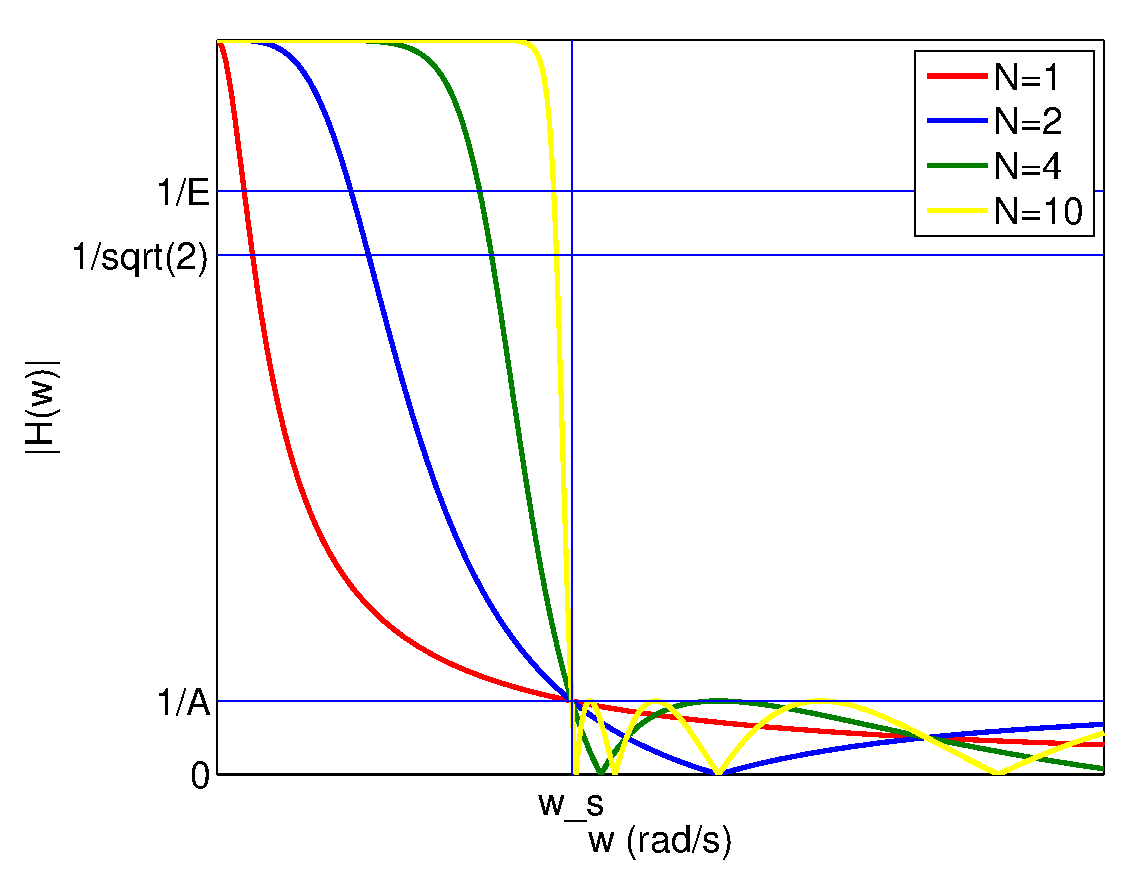
\includegraphics[width=3.5cm]{Figures/FiltroPB_Cheby2}
  }
  
  \visible<3->{
  \hspace{0.8cm}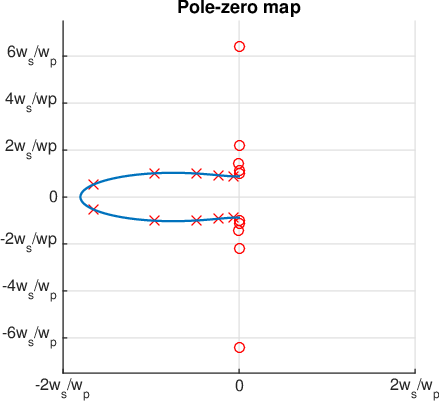
\includegraphics[width=2.2cm]{Figures/PolesCheby2.png}}
  
  \end{column}
  \end{columns}
  
  \footnotesize
  
  \vspace{0.1cm}
  
  
  
  
  
  \vspace{0.1cm}
  
  
  \footnotesize
  \begin{itemize}
  
  \visible<4->{
  
  \item Para una $\omega_s$ fija,
   si aumenta $N$ disminuye ancho de la banda de transición.
  
  
  }
  
  \visible<5->{
   \item Determinar el filtro de menor $N$ para valores dados de  $\omega_p$, $\omega_s$, $\alpha_p$, $\alpha_s$.
   }
   \vspace{0.1cm}
   {
  
   \color{gray}
  
   \scriptsize
  
   \vspace{-0.1cm}
  
   \visible<6->{
      $\!\!\!\!\left . \begin{array}{l}
    \alpha_p=-20 log_{10} \frac{1}{E} \\ \alpha_s=-20 log_{10} \frac{1}{A}\end{array}\right \}$ }   \visible<7->{ $\rightarrow \displaystyle\left . \begin{array}{l}
  E= 10^{\frac{ \alpha_p}{20}} \\ A=10^{\frac{ \alpha_s}{20}} \end{array}\right \}$ $\rightarrow \epsilon=\sqrt{E^2-1}$ }
  
  \vspace{-0.3cm}
  
   \visible<6->{
   $
   |H(j\omega_s)|^2=\frac{1}{1+\epsilon^2 \frac{cosh^2( N\cdot acosh(\omega_s/\omega_p))}{cos^2(N\cdot acos(1))}}=\frac{1}{A^2} \rightarrow$}   \visible<8->{\alert{$
  N=\frac{acosh \left ( \frac{\sqrt{A^2-1}}{\epsilon} \right)}{acosh(\omega_s/\omega_p)} $} $\rightarrow N=\frac{acosh \frac{1}{k_1}}{acosh\frac{1}{k}} $
    }
  
   }
  
  \end{itemize}
  \end{frame}


%%%%%%%%%%%%%%%%%%%%%%%%%%%%%%%

\begin{frame}\frametitle{Filtro de Chebyshev Tipo II (ejemplo)}
  
  \begin{itemize}{\scriptsize
    \item \color{olivegreen} Determinar el filtro de Chebyshev tipo II de orden más bajo con una atenuación en la banda de paso máxima de 1dB a 1KHz y una atenuación mínima en la banda de supresión de 40dB a 5KHz.
  
    \begin{columns}[T]
      \hspace{0.7cm}\begin{column}{7.1cm}
        \color{gray}
        
        \visible<1->{
        
        $\begin{array}{l}\!\!\!\left .\begin{array}{l}\omega_p=2\pi*1000\\
        \omega_s=2\pi*5000\\
        \alpha_p=1dB\\
        \alpha_s=40\end{array}\!\!\!\right \} \rightarrow\\ \: \\ \: \end{array}$ } $\!\!\!\!\!\!\begin{array}{l}E= 10^{\frac{ \alpha_p}{20}}=1.122 \\ A=10^{\frac{ \alpha_s}{20}}=100\\ \epsilon=\sqrt{E^2-1}=0.5088 \\
        N\!=\!\frac{acosh \!\left (\! \frac{\sqrt{A^2-1}}{\epsilon}\! \right)}{acosh(\omega_s/\omega_p)} \!=\!2.61 \rightarrow 3 \end{array}$
      \end{column}
      \hspace{-0.9cm}\begin{column}{4cm}
        \vspace{-0.2cm}
        \visible<2->{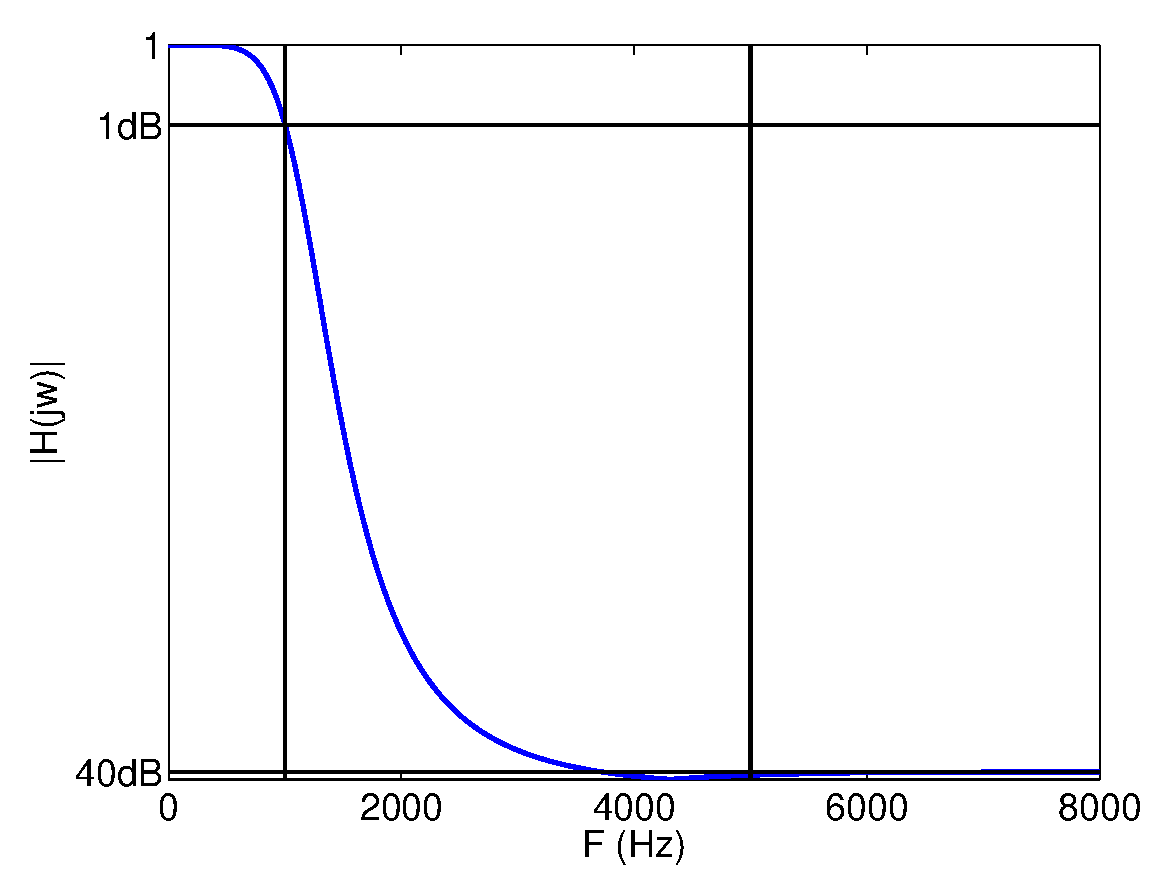
\includegraphics[width=4cm]{./Figures/FiltroPB_Cheby2Ex.eps}}
      \end{column}
    \end{columns}
  }
  \visible<3->{\vspace{-0.5cm}\footnotesize
  \item Con Matlab:
  
  \begin{itemize}
    \item \alert{\texttt{[N,wc]=cheb2ord(wp,ws,ap,as,'s')}}
    \begin{itemize}
      \color{gray}
      \item Calcula el orden \texttt{N} del filtro y la frecuencia de corte \texttt{wc}.
      \item \texttt{wp}, \texttt{ws} en rad/s.
      \item \texttt{ap}, \texttt{as} en dB.
      \item 's' para que calcule los valores del filtro de continuo.
    \end{itemize}
      \item \alert{\texttt{[B,A]=cheby2(N,as,wc,'low','s')}}
    \begin{itemize}
      \color{gray}
      \item Calcula el numerador \texttt{B} y denominador \texttt{A} de $H(s)$.
    \end{itemize}
    \item \alert{\texttt{[Hw,w]=freqs(B,A)}}
    \begin{itemize}
      \color{gray}
      \item Calcula la $H(j\omega)$ del filtro para las frecuencias \texttt{w}.
    \end{itemize}  
  \end{itemize}
  }
  \end{itemize}
  
\end{frame}
  
  
%%%%%%%%%%%%%%%%%%%%%%%%%%%%%%%%%%%%
  

  \begin{frame}
      \frametitle{Filtro Elíptico - I}
      
       \vspace{-0.2cm}
      
      \begin{columns}[T]
      \hspace{0.3cm}\begin{column}{7.5cm}
      
      \footnotesize
      
      
      \visible<1->{
      
      \hspace{0.3cm}\alert{$\displaystyle |H(jw)|^2\!=\!\frac{1}{1\!+\!\epsilon^2 R_N^2(w/\omega_p)}$}
      
      \vspace{0.1cm}
      
      \hspace{0.3cm}$R_N(w)=\frac{num(w)}{den(w)}$\hspace{1cm}$R_N(1/w)=1/R_N(w)$
      
      \vspace{0.1cm}
      
      \hspace{0.3cm}Raices $num(w)$  estan en $0<w<1$
      
      \vspace{0.1cm}
      
      \hspace{0.3cm}Raices $den(w)$ estan en $1<w<\infty$
      
      
      }
      
      \vspace{0.1cm}
      
      \hspace{0.3cm}\alert{$\displaystyle  H(s)=E_0\frac{ K(s) \prod_{l=1}^{floor(N/2)} (s^2+\omega_{zl}^2)}{\prod_{l=1}^{N} (s-p_l)}$}
      
      
      \vspace{0.2cm}
      
      \scriptsize
      
       \hspace{0.3cm}con  $p_l\!=\!(\sigma_l\!+\!j\omega_{pl})$, $K(s)\!=\!1$ si $N$ par, $K(s)\!=\!s$  si $N$ impar
      
      
      \footnotesize
      
      \begin{itemize}
      
      \visible<2->{
      
      \item Para una $\omega_p$ fija,
       si aumenta $N$ disminuye ancho de la banda de transición.
      
      
      }
      
      
      
      \visible<3->{
       \item Determinar el filtro de menor $N$ para valores dados de  $\omega_p$, $\omega_s$, $\alpha_p$, $\alpha_s$.
       }
      
      \end{itemize}
      
      
      \end{column}
      \hspace{-0.3cm}\begin{column}{4cm}
      \visible<1->{
      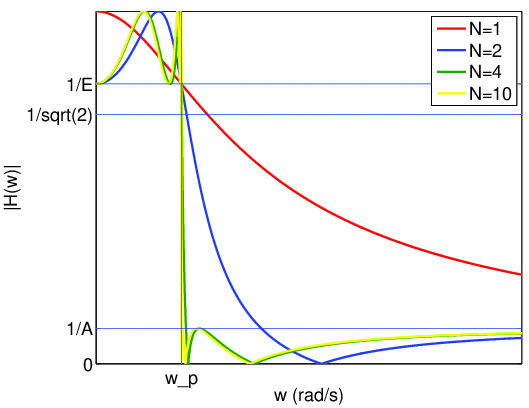
\includegraphics[width=3.5cm]{Figures/FiltroPB_Elip.png}
      }
      
      \visible<1->{
      \hspace{0.8cm}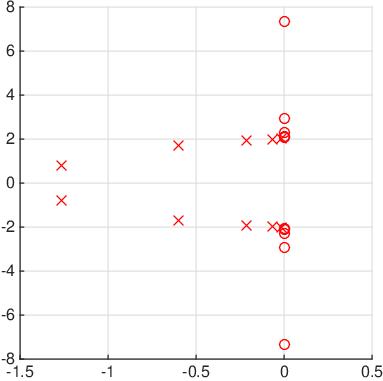
\includegraphics[width=2.5cm]{Figures/PolesEllip.png}
      }
      
      \end{column}
      \end{columns}
      
      \footnotesize
      
      \vspace{0.1cm}
      
      
      
      \footnotesize
      
      
       \vspace{0.1cm}
       {
      
       \color{gray}
      \visible<4->{
      \hspace{0.8cm}$\alpha_p=-20 log_{10} \frac{1}{E}$, \hspace{0.4cm}$\alpha_s=-20 log_{10}$,  \hspace{0.4cm}$k_1=\frac{\epsilon}{\sqrt{A^2-1}}$, \hspace{0.4cm}$ N= \frac{2log_{10}(4/k_1)}{log_{10}(1/\rho)}$
      
      \hspace{0.8cm}$\rho\!=\!\rho_0\!+\!2\rho_0^5\!+\!15\rho_0^9\!+\!150\rho_0^{13}$, \hspace{0.4cm}$\rho_0=\frac{1-\sqrt{k'}}{2(1+\sqrt{k'})}$, \hspace{0.4cm}$k'=\sqrt{1-k^2}$,\hspace{0.4cm}$k=\frac{\omega_p}{\omega_s}$
      
       \vspace{0.1cm}
      
      \hspace{0.8cm}Se necesita un computador para calcular los valores de $\omega_{zl}$, $\sigma_l$ y $\omega_{pl}$
      }
      
       }
      
\end{frame}

%%%%%%%%%%%%%%%%%%%%%%%%%%%%%%%

\begin{frame}
  \frametitle{Filtro Elíptico (ejemplo)}
  
  \vspace{-0.3cm}
  
  \begin{itemize}
  
  {
  \scriptsize
  \item \color{olivegreen} Determinar el filtro elíptico de orden más bajo con una atenuación en la banda de paso máxima de 1dB a 1KHz y una atenuación mínima en la banda de supresión de 40dB a 5KHz.
  
  \begin{columns}[T]
  \hspace{1cm}\begin{column}{7cm}
  \color{gray}
  
  \color{gray}
  $\!\!\!\!\!\!\begin{array}{ll}
  \omega_p\!=\!2\pi\!*\!1000 &
   \omega_s\!=\!2\pi\!*\!5000\\
   \alpha_p=1dB&
   \alpha_s=40\\
   E= 10^{\frac{ \alpha_p}{20}}=1.122  & A=10^{\frac{ \alpha_s}{20}}=100\\ \epsilon=\sqrt{E^2-1}=0.5088 &
   k_1=\frac{\epsilon}{\sqrt{A^2-1}}=0.0051\\
   k=\frac{\omega_s}{\omega_p}=\frac{1}{5}&
   k'=\sqrt{1-k^2}=0.9798\\
   \rho_0=\frac{1-\sqrt{k'}}{2(1+\sqrt{k'})}=0.00255 \end{array}$
  
  
  $\!\!\!\rho\!=\!\rho_0\!+\!2\rho_0^5\!+\!15\rho_0^9\!+\!150\rho_0^{13}\!=\!0.002551$
  
  \vspace{0.1cm}
  
  $\!\!\!N= \frac{2log_{10}(4/k_1)}{log_{10}(1/\rho)}=2.23  \rightarrow 3$
  
   \end{column}
  \hspace{-1cm} \begin{column}{4cm}
  
   \visible<2->{ 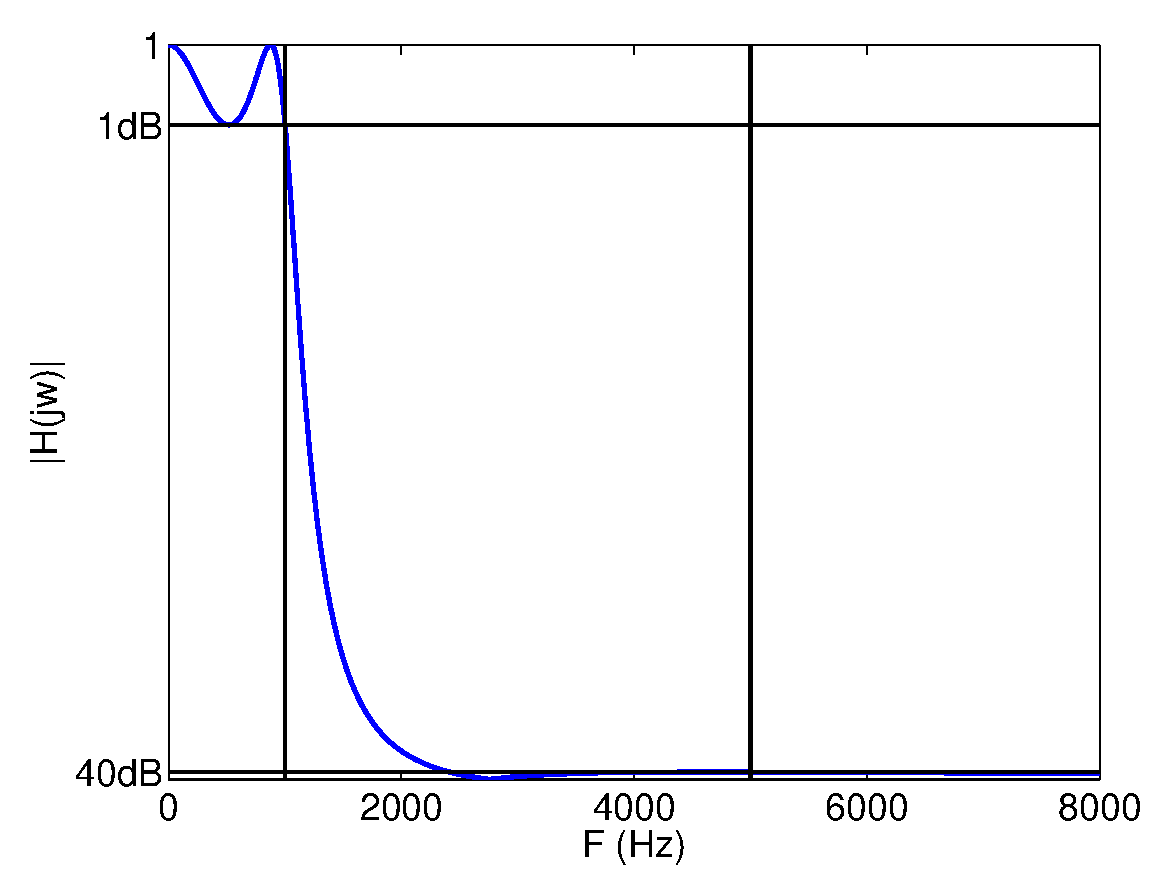
\includegraphics[width=4cm]{./Figures/FiltroPB_EllipEx.eps}}
  
   \end{column}
   \end{columns}
  
  }
  \visible<3->{
  {
  
  \vspace{0.1cm}
  
  \footnotesize
  \item Con Matlab:
  
  \vspace{-0.1cm}
  
  \begin{itemize}
  \item \alert{\texttt{[N,wp]=ellipord(wp,ws,ap,as,'s')}}
  \begin{itemize}
  \color{gray}
  \item Calcula el orden del filtro $N$ y la $\omega_p$.
  \item \texttt{wp}, \texttt{ws} en rad/s.
  \item \texttt{ap}, \texttt{as} en dB.
  \item 's' para que calcule los valores del filtro de continuo.
  \end{itemize}
  \item \alert{\texttt{[B,A]=ellip(N,as,ap,wp,'low','s')}}
  \begin{itemize}
  \color{gray}
  \item Calcula el numerador \texttt{B} y denominador \texttt{A} de $H(s)$.
  \end{itemize}
  \end{itemize}
  }
  }
  \end{itemize}
  
\end{frame}

\begin{frame}\frametitle{Resumen de filtro paso bajo: ordenes de Matlab}

  \begin{itemize}
    \item Cálculo del orden y frecuencia característica del filtro:
    \begin{itemize}
      \item \alert{\texttt{[N,wc]=buttord(wp,ws,ap,as,'s')}}
      \item \alert{\texttt{[N,wc]=cheb1ord(wp,ws,ap,as,'s')}}
      \item \alert{\texttt{[N,wc]=cheb2ord(wp,ws,ap,as,'s')}}
      \item \alert{\texttt{[N,wc]=ellipord(wp,ws,ap,as,'s')}}
    \end{itemize}
      \item Cálculo de la función de transferencia del filtro, $H(s)$:
    \begin{itemize}
      \item \alert{\texttt{[B,A]=butter(N,wc,'low','s')}}
      \item \alert{\texttt{[B,A]=cheby1(N,ap,wc,'low','s')}}
      \item \alert{\texttt{[B,A]=cheby2(N,ap,wc,'low','s')}}
      \item \alert{\texttt{[B,A]=ellip(N,ap,as,wc,'low','s')}}
    \end{itemize}
      \item Cálculo y representación del espectro del filtro, $H(j\omega)$.
    \begin{itemize}
      \item \alert{\texttt{[Hw,w]=freqs(B,A)}}
      \item \alert{\texttt{plot(w,abs(Hw))}}
      \item \alert{\texttt{plot(w,angle(Hw))}}
      \item \alert{\texttt{plot(w,unwrap(angle(Hw)))}}
    \end{itemize}
  \end{itemize}

\end{frame}


%%%%%%%%%%%%%%%%%%%%%%%%%%%%%%%%%%%%%%%%


\subsection{Filtro paso alta, paso banda y supresores de banda}

% \begin{frame}
% \frametitle{Filtro paso alta, paso banda y supresores de banda I}

% \footnotesize
% \begin{itemize}
% \item Las funciones de transferencia $H(\hat s)$ de los filtros  paso alta, paso banda y supresores de banda se pueden obtener a partir de la función de transferencia de un filtro paso baja $H_{LP}(s)$ a través de una transformación espectral $s=F(\hat s)$.
% \begin{itemize}
% \footnotesize
% \visible<2->{
% \item Filtro paso alta: \hspace{1.3cm}$s=\frac{\omega_p \hat \omega_p}{\hat s}$ \hspace{1.5cm} $- w \hat w=\omega_p \hat \omega_p$}
% \visible<3->{
% \item Filtro paso banda: \hspace{1.0cm} $s=\omega_p\frac{\hat s^2+\hat \omega_0^2}{\hat s (\hat \omega_{p2}-\hat \omega_{p1})}$
% \hspace{0.5cm}$w=\omega_p\frac{\hat w^2-\hat \omega_0^2}{\hat w (\hat \omega_{p2}-\hat \omega_{p1})}$

% \hspace{3.7cm}$\hat \omega_0^2=\hat \omega_{p1}\hat \omega_{p2}=\hat \omega_{s1}\hat \omega_{s2}$}

% \visible<4->{

% \item Filtro supresor de banda : $s=\omega_s\frac{\hat s (\hat \omega_{s2}-\hat \omega_{s1})}{\hat s^2+\hat \omega_0^2}$ \hspace{0.5cm}$w=\omega_s\frac{\hat w (\hat \omega_{s2}-\hat \omega_{s1})}{\hat \omega_0^2-\hat w^2}$

% \hspace{3.7cm}$\hat \omega_0^2=\hat \omega_{p1}\hat \omega_{p2}=\hat \omega_{s1}\hat \omega_{s2}$

% }

% \end{itemize}

% \visible<5->{
% \item Se cogen las especificaciones del filtro en que hay que hacer, y se calculan las correspondientes al filtro paso baja con las fórmulas de la frecuencia (suponiendo que $\omega_p=1$). }
% \visible<6->{
% \item Acto seguido se calcula la función de transferencia del filtro paso baja asociado al filtro paso baja.}
% \visible<7->{
% \item La función de transferencia del filtro destino será $H(\hat s)=H_{LP}(s=F(\hat s))$ con la $F(\hat s)$ del filtro correspondiente  correspondiente}
% \end{itemize}

% \end{frame}

% %%%%%%%%%%%%%%%%%%%%%%%%%%%%%%%
% % Transformaciones Espectrales
% %%%%%%%%%%%%%%%%%%%%%%%%%%%%%%%
  

% \begin{frame}{Transformaciones espectrales}
%   \begin{columns}
%       \begin{column}{0.45\textwidth}
%           \centering\small
%           Paso bajo $\rightarrow$ Paso alto\\
%           \[s=\frac{\omega_p\hat{\omega}_p}{\hat{s}}\Leftrightarrow\omega=\frac{-\omega_p\hat{\omega}_p}{\hat{\omega}}\]
%       \end{column}
%       \begin{column}{0.55\textwidth}
%           \centering
%           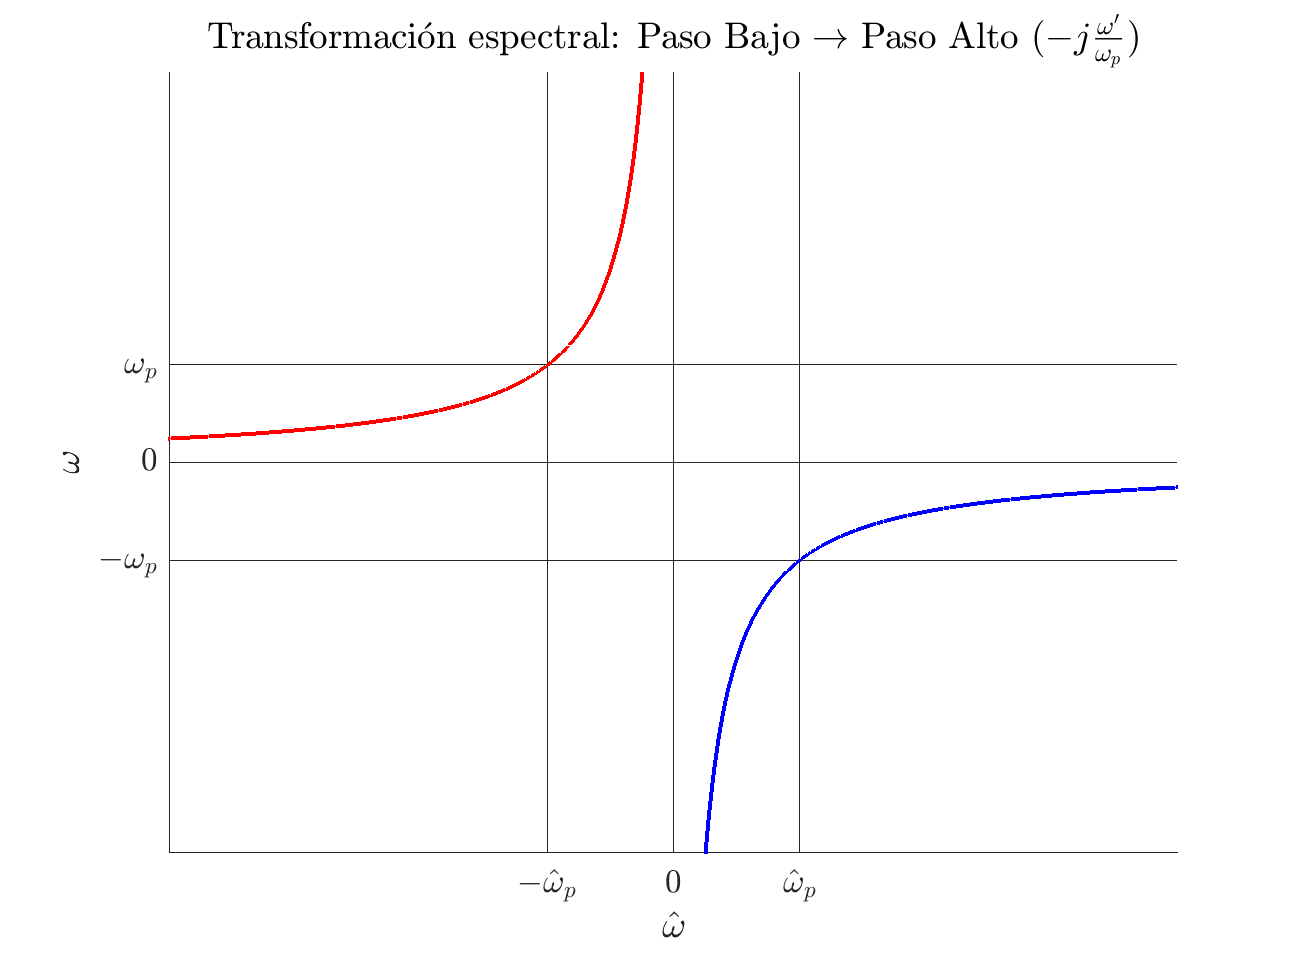
\includegraphics[height=4cm]{Figures/TE_1a.png}\\
%       \end{column}
%   \end{columns}
%   \begin{center}
%       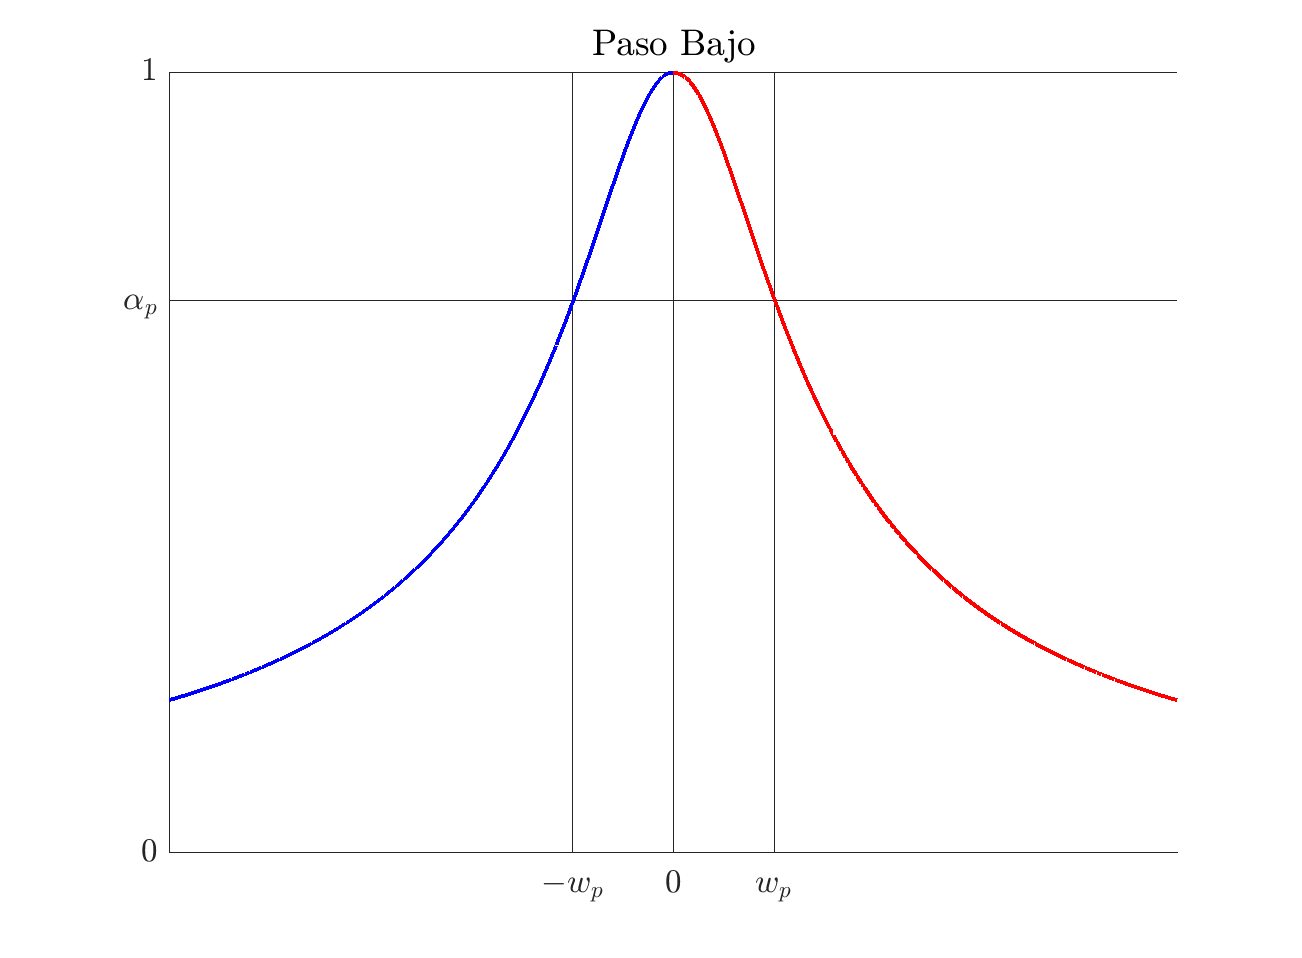
\includegraphics[height=4.25cm]{Figures/TE_1b.png}%
%       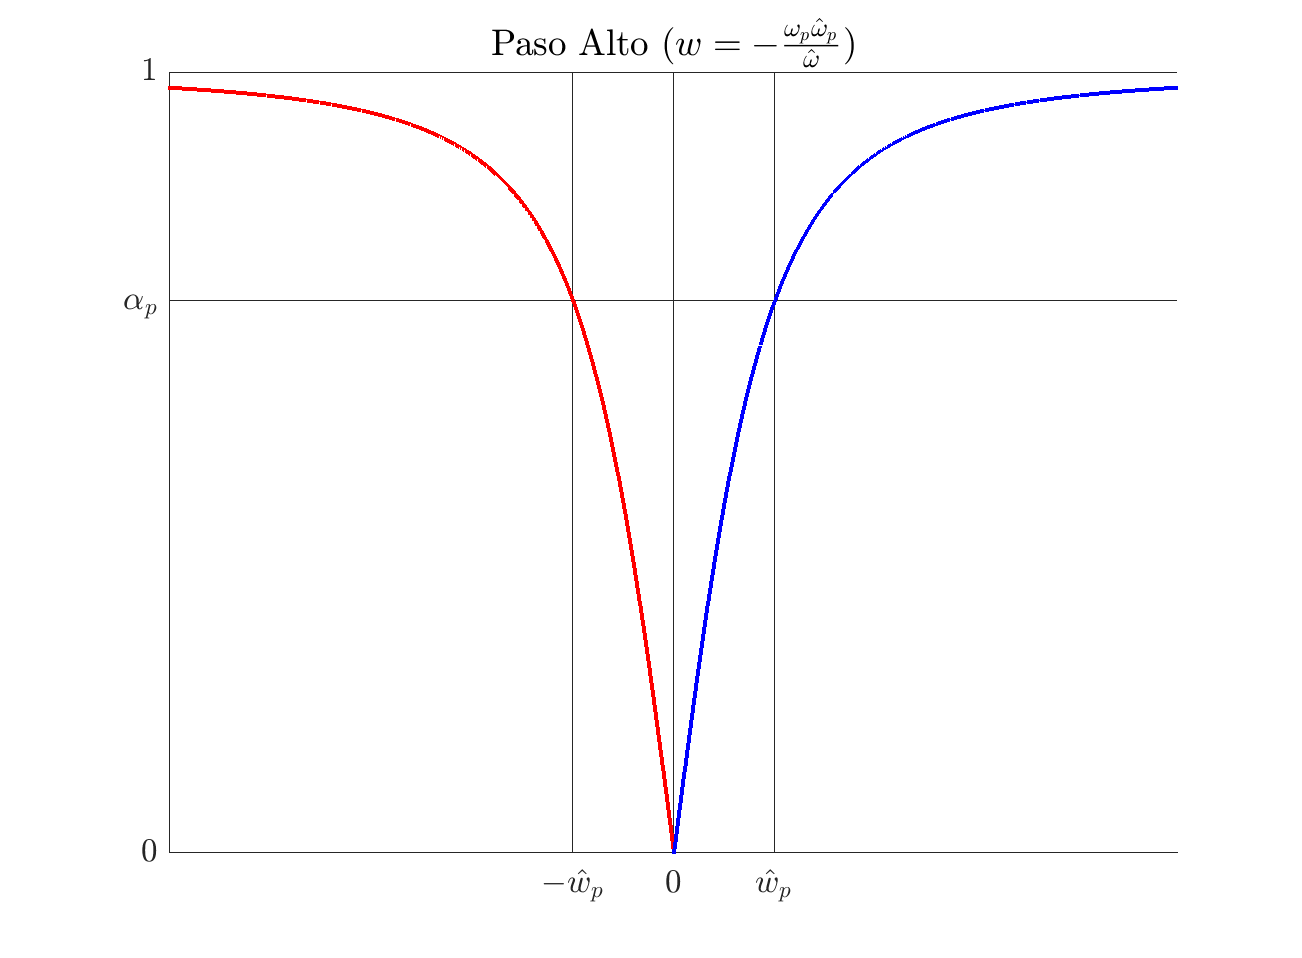
\includegraphics[height=4.25cm]{Figures/TE_1c.png}
%   \end{center}
% \end{frame}

% \begin{frame}{Transformaciones espectrales}
% \begin{columns}
%   \begin{column}{0.45\textwidth}
%       \centering\footnotesize
%       Paso bajo $\rightarrow$ Paso banda\\
%       \[s=\frac{\omega_p(\hat{s}^2+\hat{\omega_0}^2)}{\hat{s}(\hat{\omega}_{p_2}-\hat{\omega}_{p_1})} \Leftrightarrow
%       \omega=\frac{\omega_p(\hat{\omega}^2-\hat{\omega}_0^2)}{\hat{\omega}(\hat{\omega}_{p_2}-\hat{\omega}_{p_1})}\]\\
%   \end{column}
%   \begin{column}{0.55\textwidth}
%       \centering
%       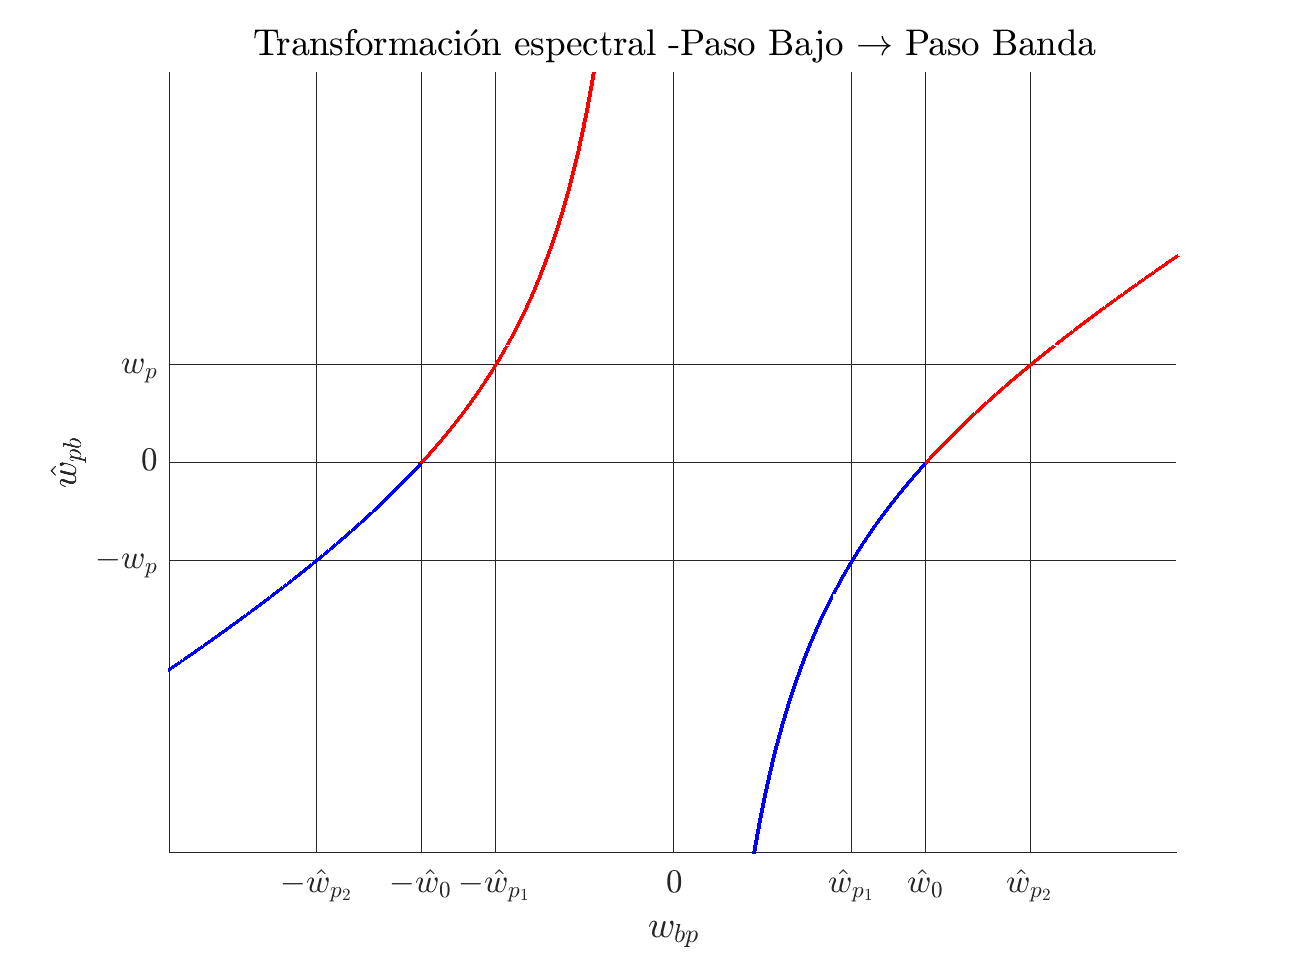
\includegraphics[height=4cm]{Figures/TE_2a.png}\\
%   \end{column}
% \end{columns}
% \begin{center}
%   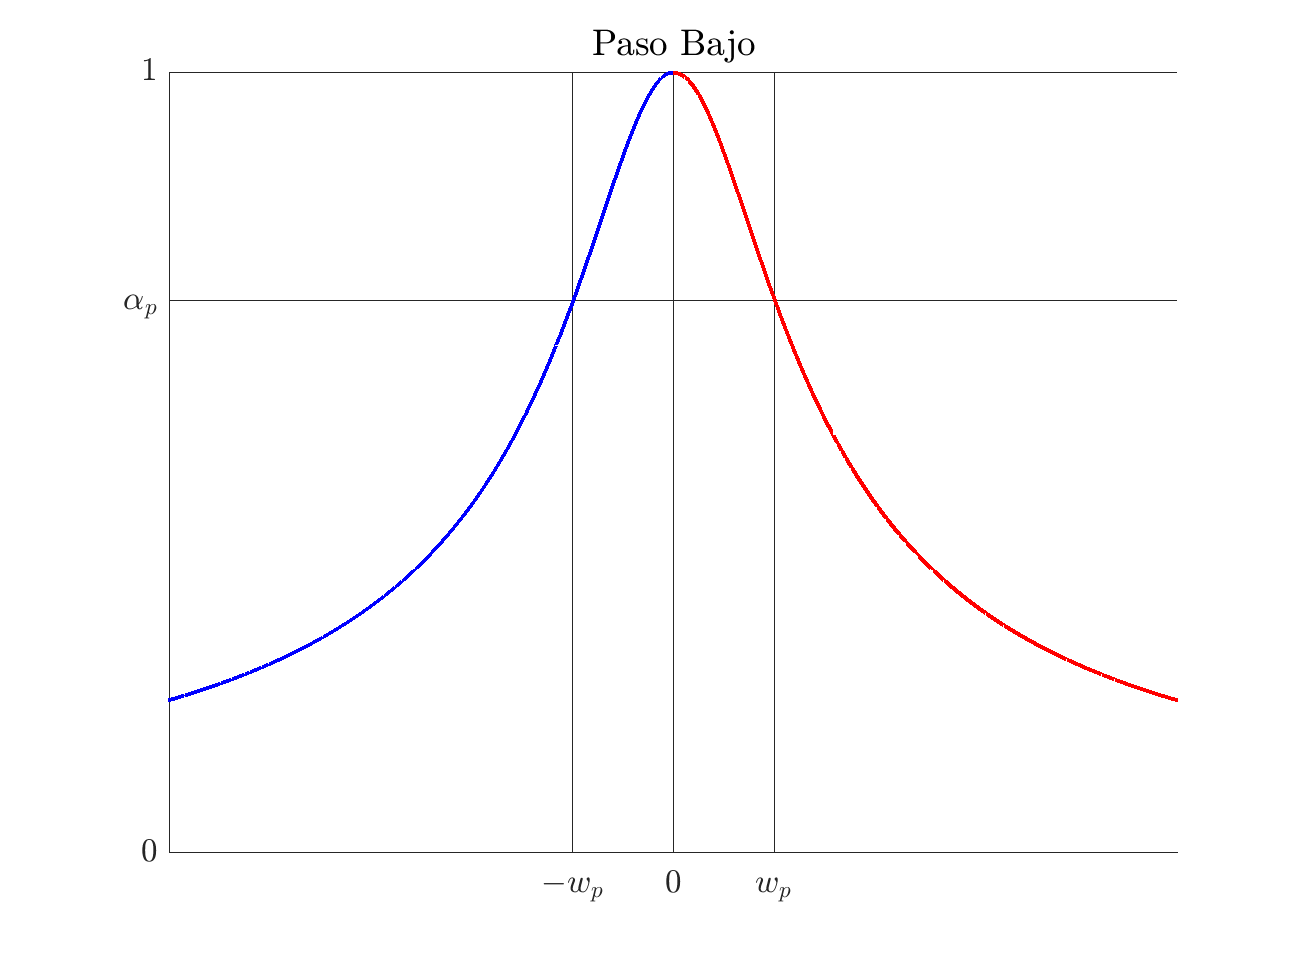
\includegraphics[height=4.25cm]{Figures/TE_2b.png}%
%   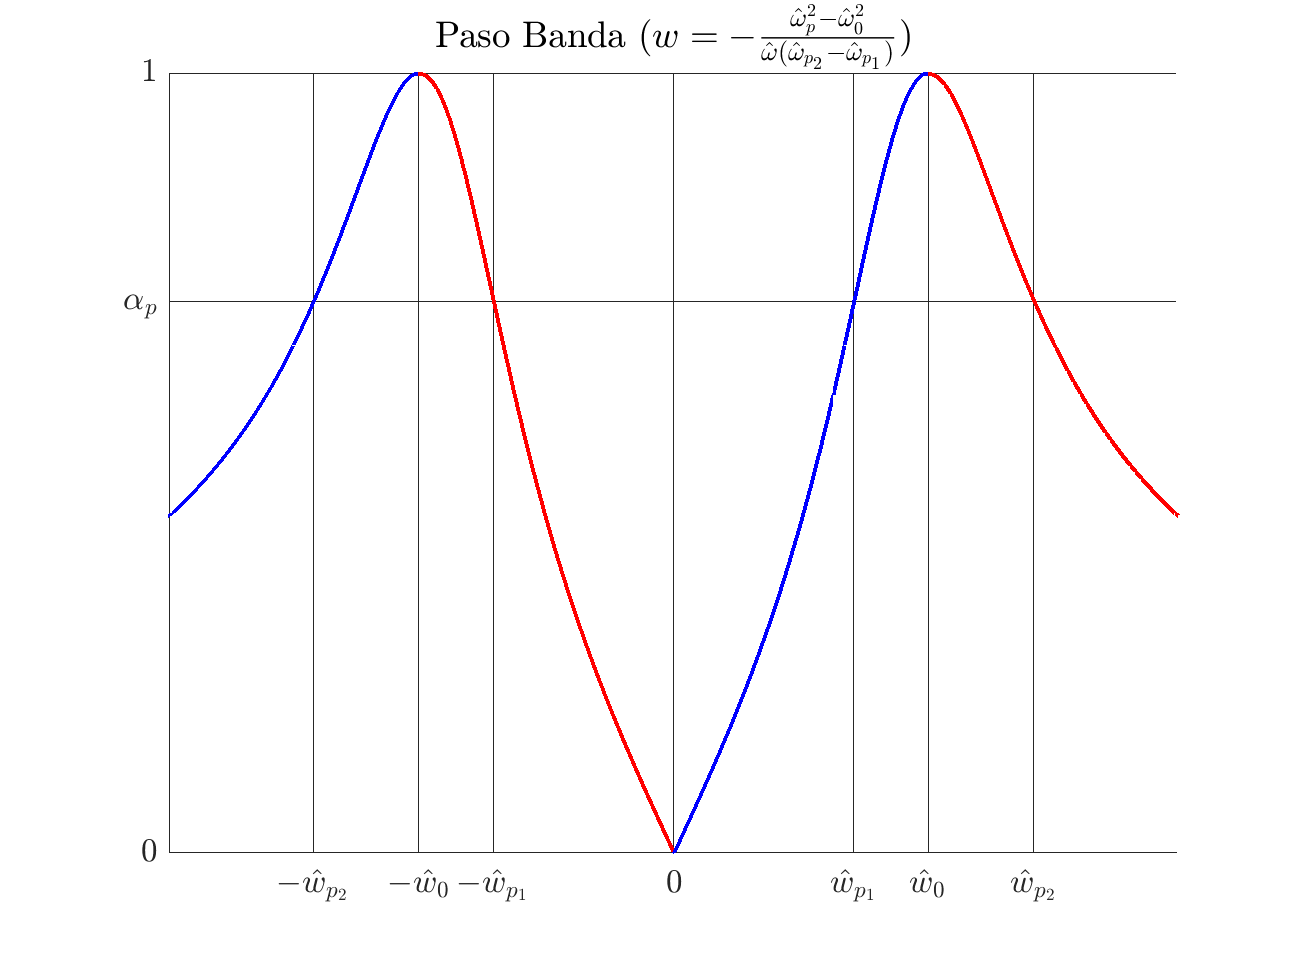
\includegraphics[height=4.25cm]{Figures/TE_2c.png}
% \end{center}
% \end{frame}

% \begin{frame}{Transformaciones espectrales}
% \begin{columns}
%   \begin{column}{0.45\textwidth}
%       \centering\footnotesize
%       Paso bajo $\rightarrow$ Supresor de banda\\
%       \[s=\omega_s\frac{\hat{s}(\hat{\omega}_{s_2}-\hat{\omega}_{s_1})}{\hat{s}^2+\hat{\omega_0}^2}\Leftrightarrow\omega=\omega_s\frac{\hat{\omega}(\hat{\omega}_{s_2}-\hat{\omega}_{s_1})}{\hat{\omega_0}^2-\hat{\omega}^2}\]\\
%   \end{column}
%   \begin{column}{0.55\textwidth}
%       \centering
%       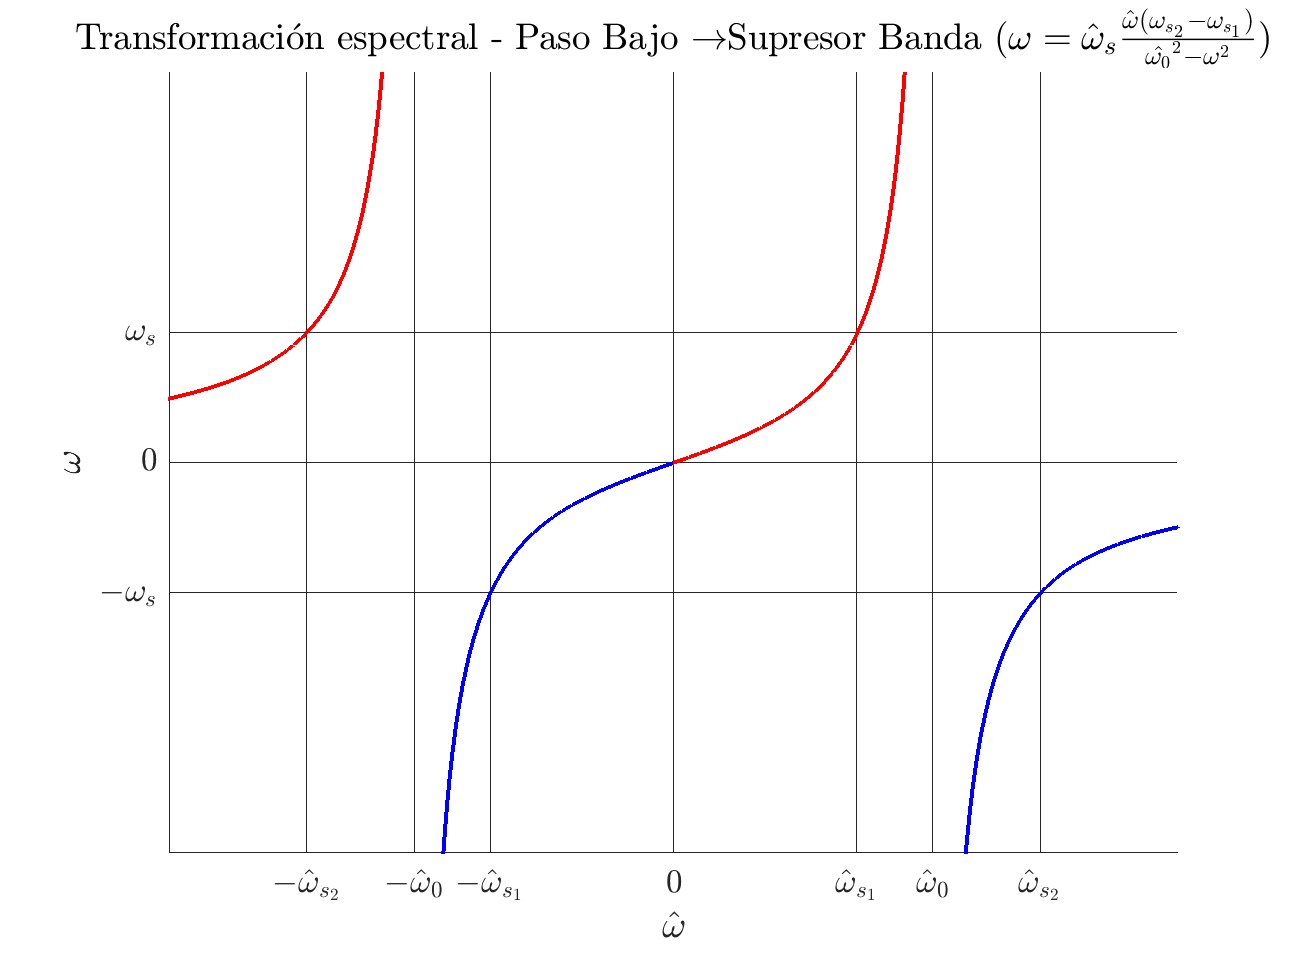
\includegraphics[height=4cm]{Figures/TE_3a.png}\\
%   \end{column}
% \end{columns}
% \begin{center}
%   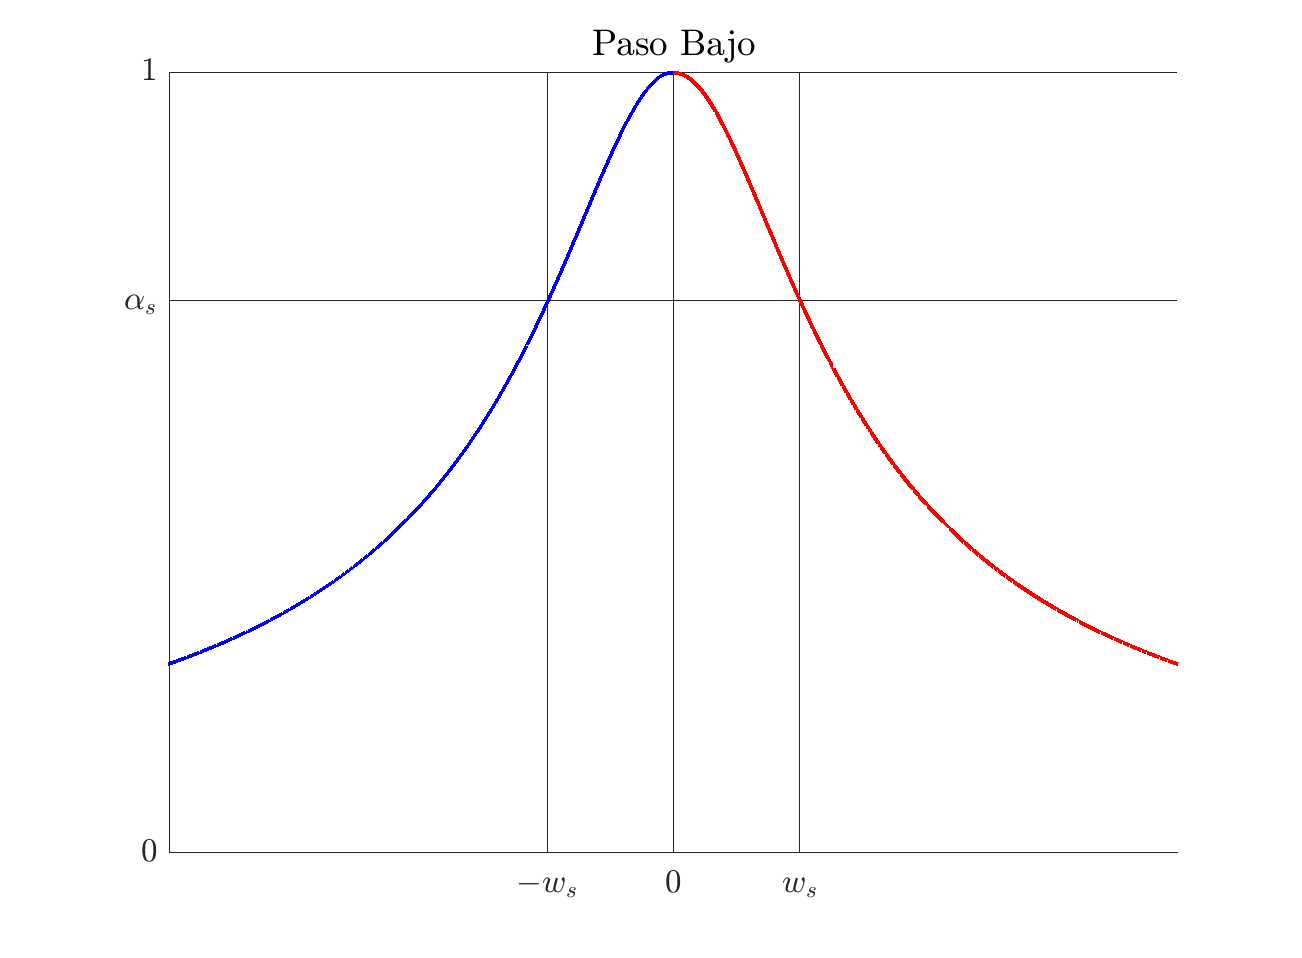
\includegraphics[height=4.25cm]{Figures/TE_3b.png}%
%   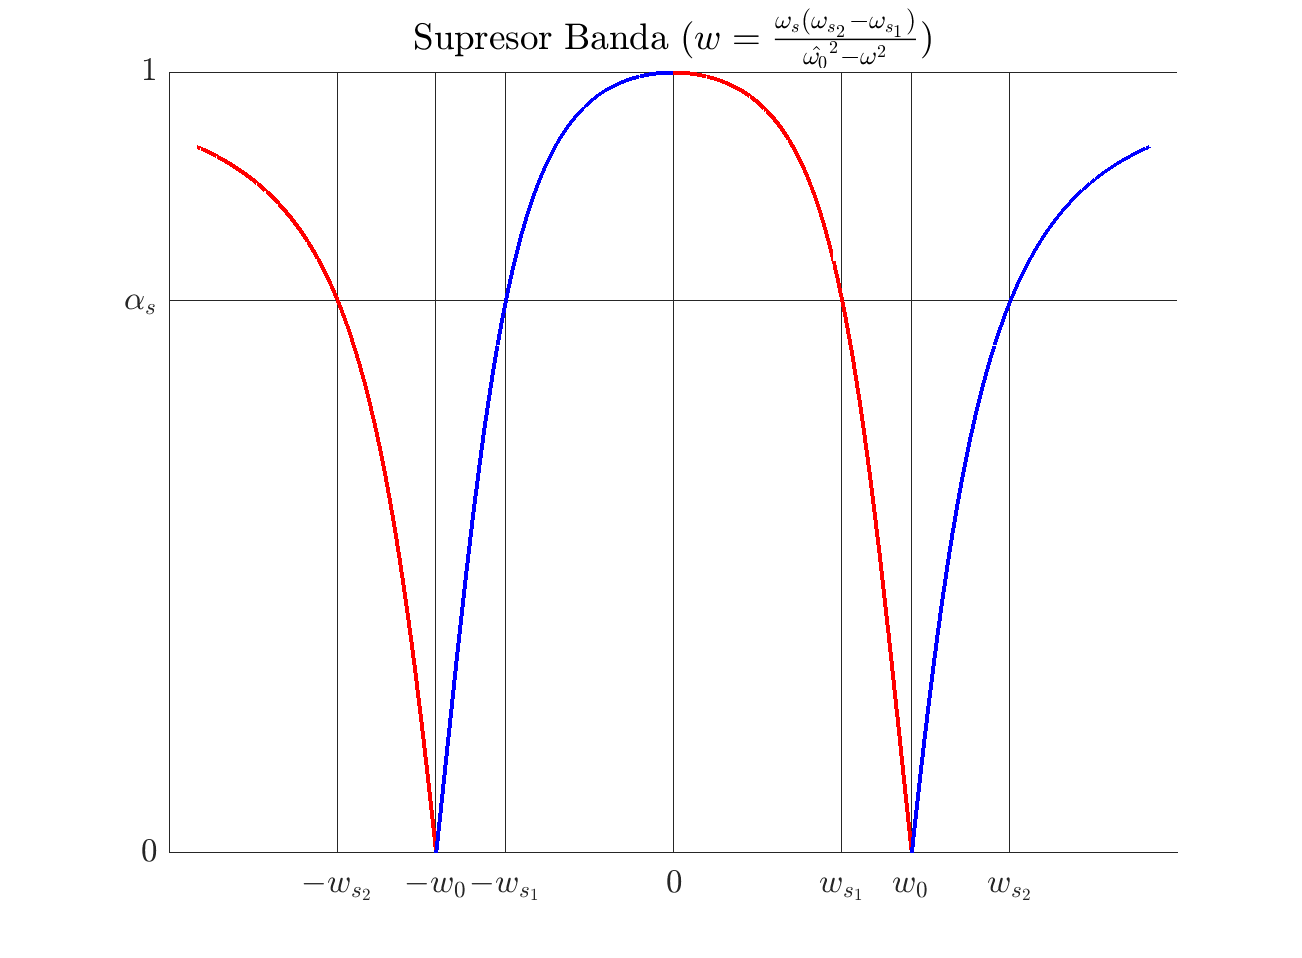
\includegraphics[height=4.25cm]{Figures/TE_3c.png}
% \end{center}
% \end{frame}

%%%%%%%%%%%%%%%%%%%%%%%%%%%%%%%%%%%%%%%%%%%
% \subsection{Filtro paso alta, paso banda y supresores de banda}

\begin{frame}
\frametitle{Filtro paso alta, paso banda y supresores de banda I}

  \footnotesize
  \begin{itemize}
  \item Las funciones de transferencia $H(\hat s)$ de los filtros  paso alta, paso banda y supresores de banda se pueden obtener a partir de la función de transferencia de un filtro paso baja $H_{LP}(s)$ a través de una transformación espectral $s=F(\hat s)$.
  \begin{itemize}
    \footnotesize
    \item Filtro paso alta: \hspace{1.3cm}$s=\frac{\omega_p \hat \omega_p}{\hat s}$ \hspace{1.5cm} $-\omega \hat \omega=\omega_p \hat \omega_p$
    \item Filtro paso banda: \hspace{1.0cm} $s=\omega_p\frac{\hat s^2+\hat \omega_0^2}{\hat s (\hat \omega_{p2}-\hat \omega_{p1})}$
    \hspace{0.5cm}$\omega=\omega_p\frac{\hat\omega^2-\hat \omega_0^2}{\hat \omega (\hat \omega_{p2}-\hat \omega_{p1})}$

    \hspace{3.7cm}$\hat \omega_0^2=\hat \omega_{p1}\hat \omega_{p2}=\hat \omega_{s1}\hat \omega_{s2}$
    \item Filtro supresor de banda : $s=\omega_s\frac{\hat s (\hat \omega_{s2}-\hat \omega_{s1})}{\hat s^2+\hat \omega_0^2}$ \hspace{0.5cm}$\omega=\omega_s\frac{\hat \omega (\hat \omega_{s2}-\hat \omega_{s1})}{\hat \omega_0^2-\hat \omega^2}$

    \hspace{3.7cm}$\hat \omega_0^2=\hat \omega_{p1}\hat \omega_{p2}=\hat \omega_{s1}\hat \omega_{s2}$
  \end{itemize}

\item Pasar especificaciones del filtro deseado a paso bajo (suponiendo $\omega_p=1$).
\item Calcula la función de transferencia del filtro paso baja asociado al filtro paso baja.
\item La función de transferencia del filtro destino será $H(\hat s)=H_{LP}(s=F(\hat s))$ con la $F(\hat s)$ del filtro correspondiente
\end{itemize}

\end{frame}

\begin{frame}{Transformaciones espectrales}
  \begin{columns}
      \begin{column}{0.45\textwidth}
          \centering\small
          Paso bajo $\rightarrow$ Paso alto\\
          \[s=\frac{\omega_p\hat{\omega}_p}{\hat{s}}\Leftrightarrow\omega=\frac{-\omega_p\hat{\omega}_p}{\hat{\omega}}\]
      \end{column}
      \begin{column}{0.55\textwidth}
          \centering
          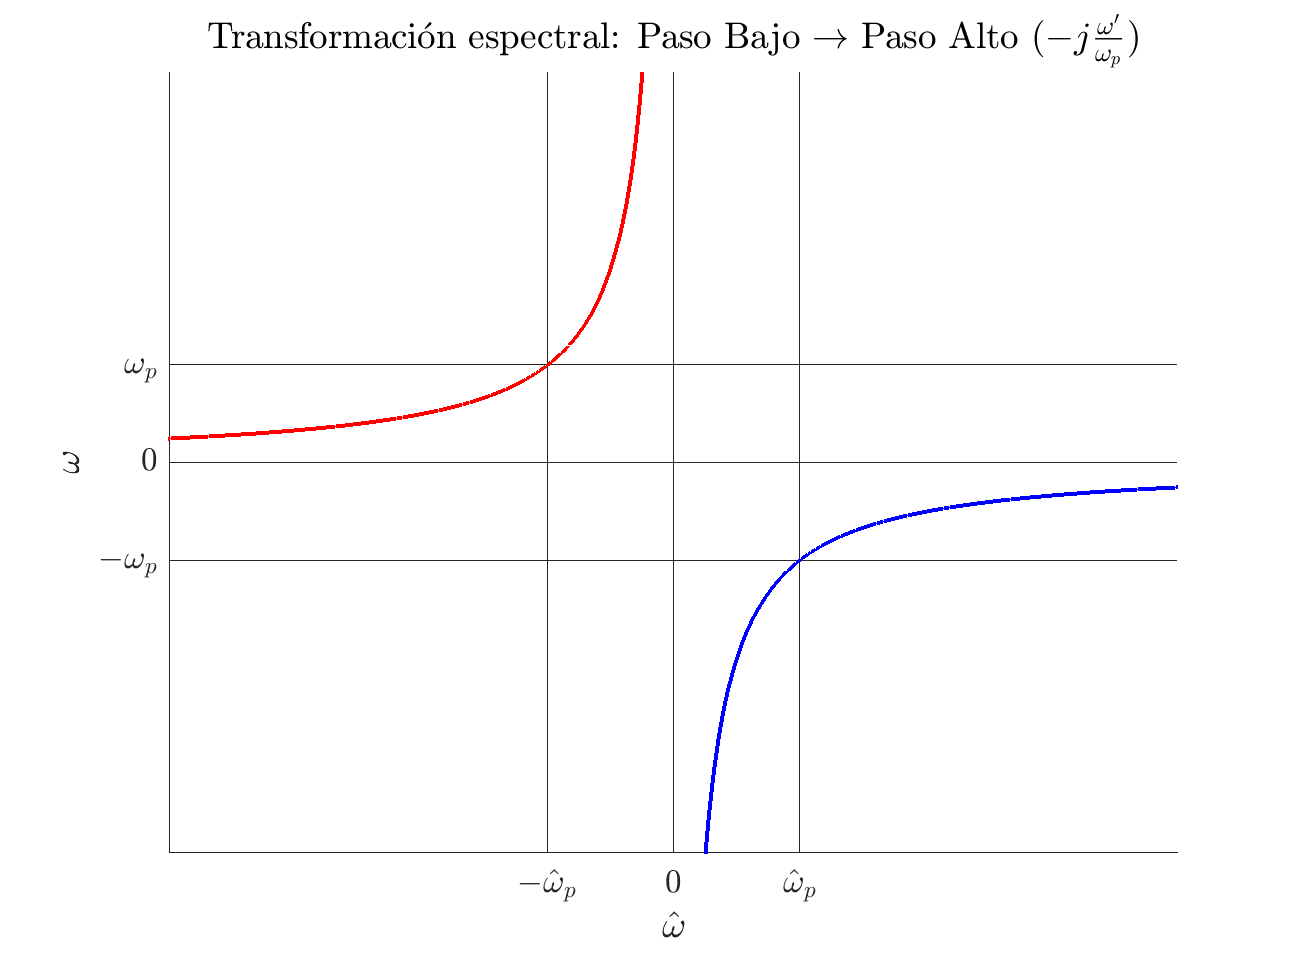
\includegraphics[height=4cm]{Figures/TE_1a.png}\\
      \end{column}
  \end{columns}
  \begin{center}
      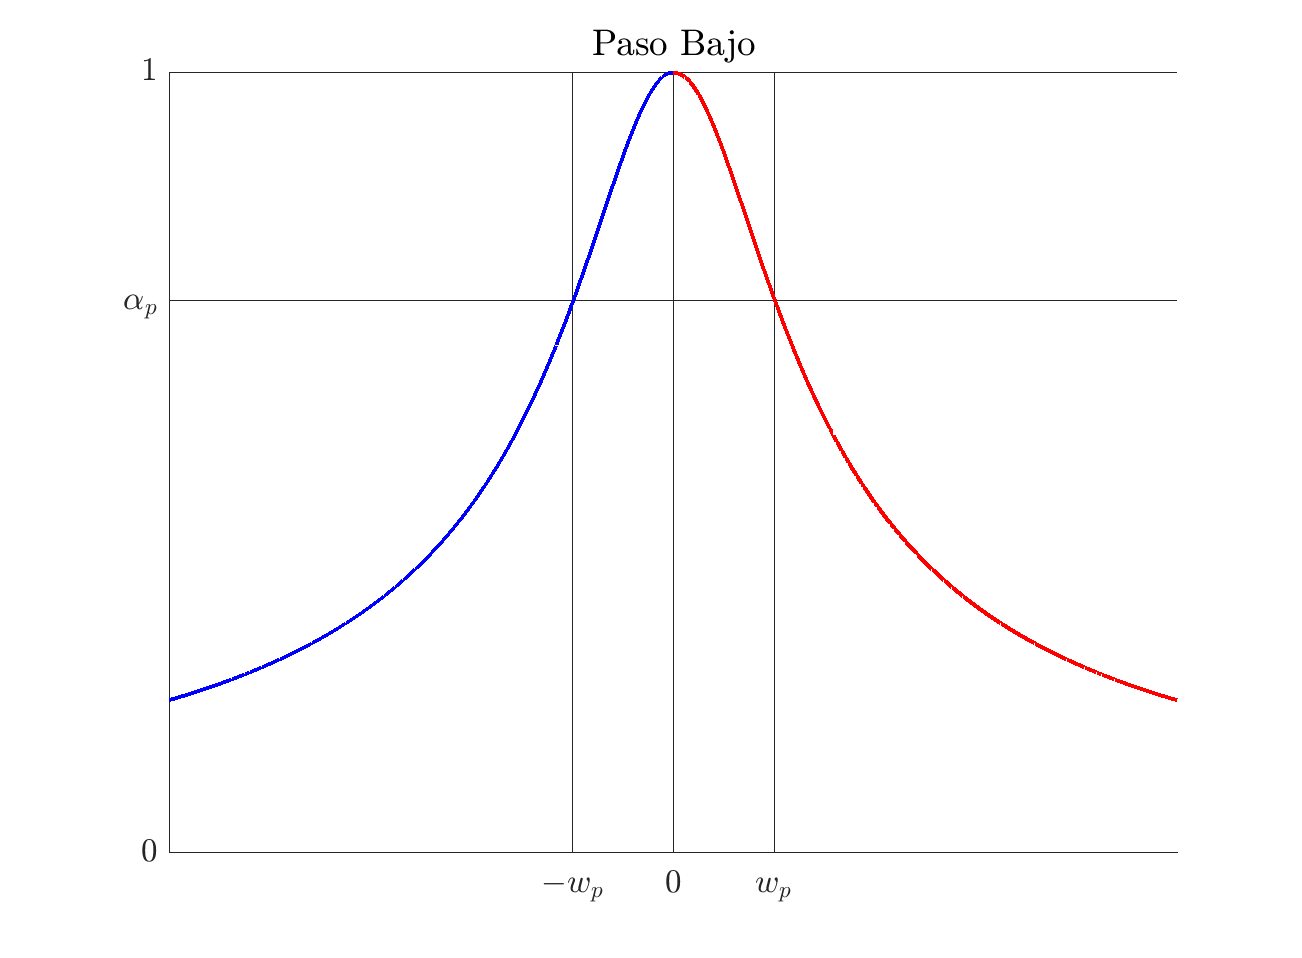
\includegraphics[height=4.25cm]{Figures/TE_1b.png}%
      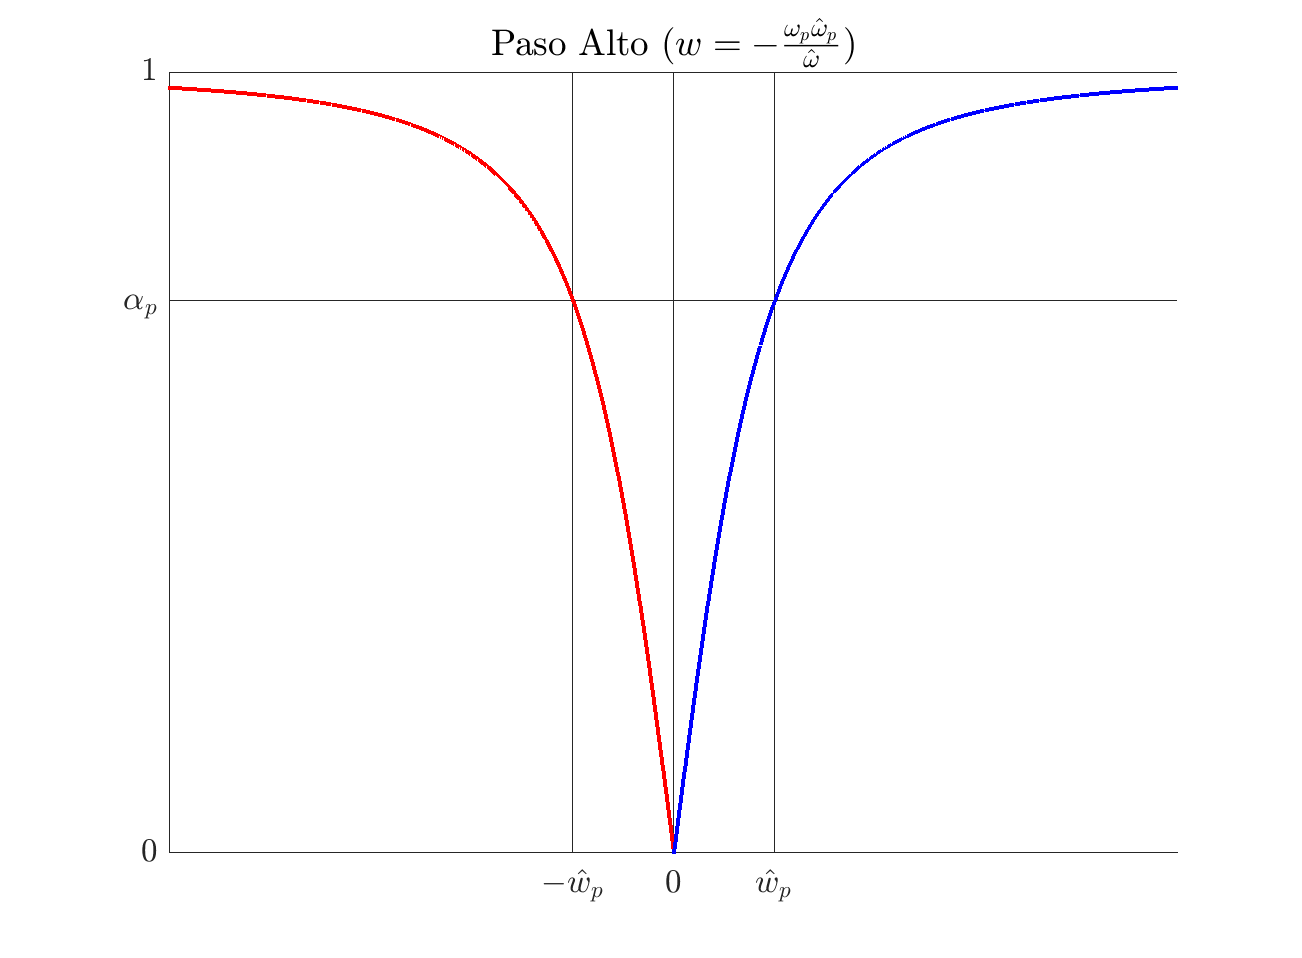
\includegraphics[height=4.25cm]{Figures/TE_1c.png}
  \end{center}
\end{frame}

\begin{frame}{Transformaciones espectrales}
\begin{columns}
  \begin{column}{0.45\textwidth}
      \centering\footnotesize
      Paso bajo $\rightarrow$ Paso banda\\
      \[s=\frac{\omega_p(\hat{s}^2+\hat{\omega_0}^2)}{\hat{s}(\hat{\omega}_{p_2}-\hat{\omega}_{p_1})} \Leftrightarrow
      \omega=\frac{\omega_p(\hat{\omega}^2-\hat{\omega}_0^2)}{\hat{\omega}(\hat{\omega}_{p_2}-\hat{\omega}_{p_1})}\]\\
  \end{column}
  \begin{column}{0.55\textwidth}
      \centering
      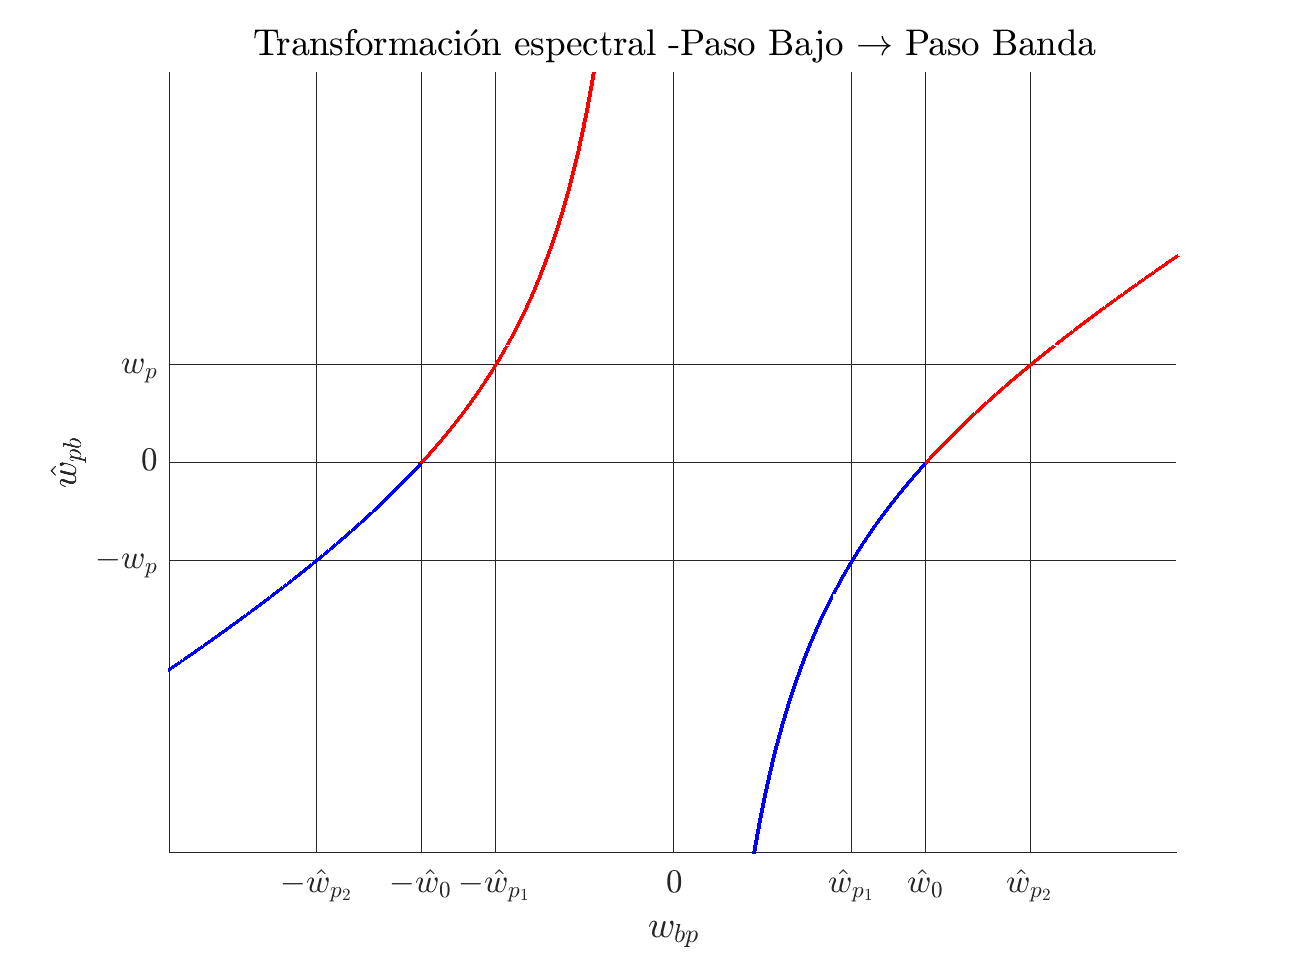
\includegraphics[height=4cm]{Figures/TE_2a.png}\\
  \end{column}
\end{columns}
\begin{center}
  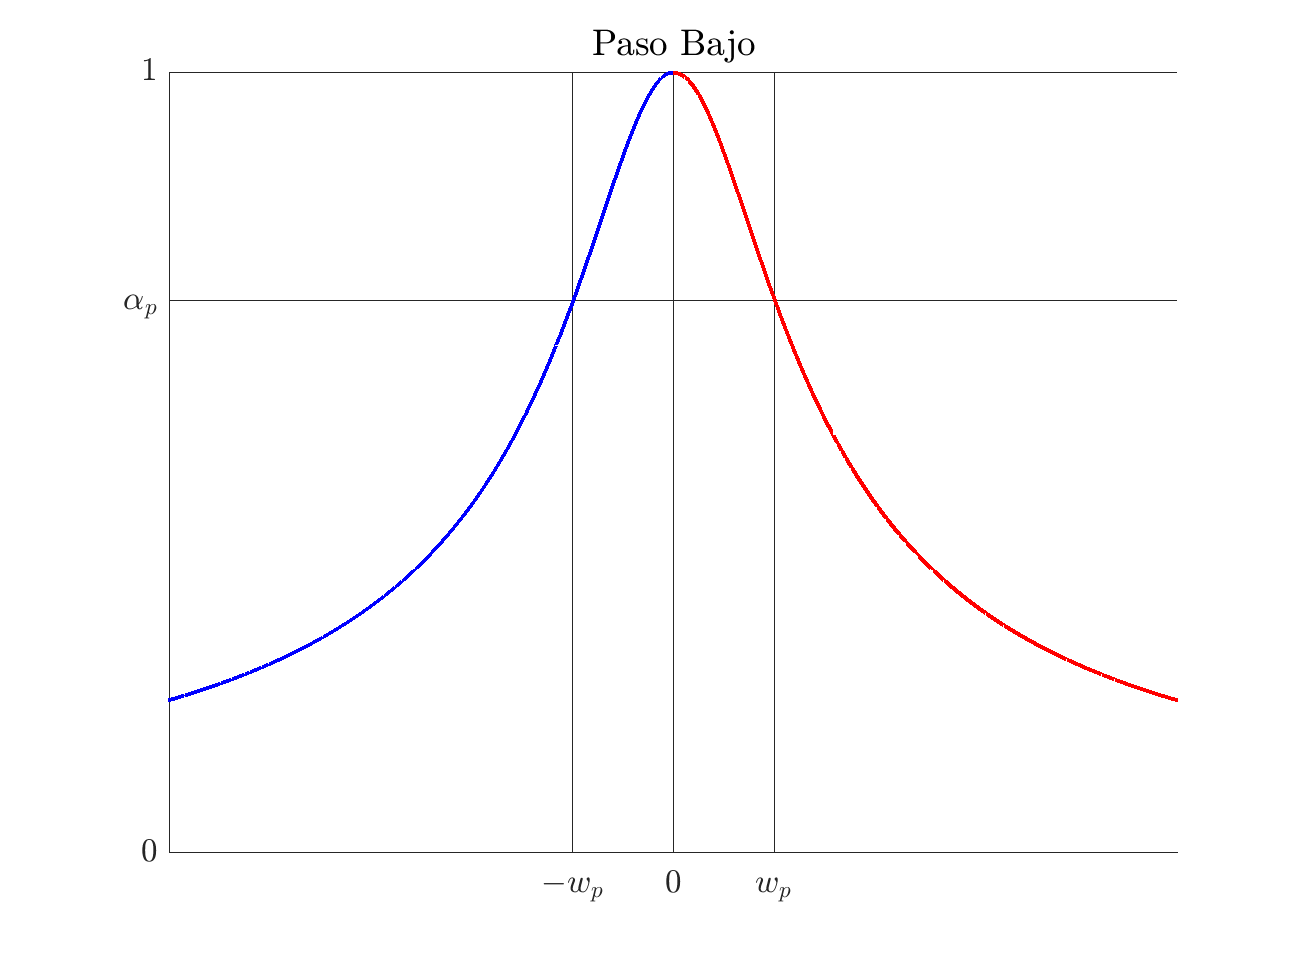
\includegraphics[height=4.25cm]{Figures/TE_2b.png}%
  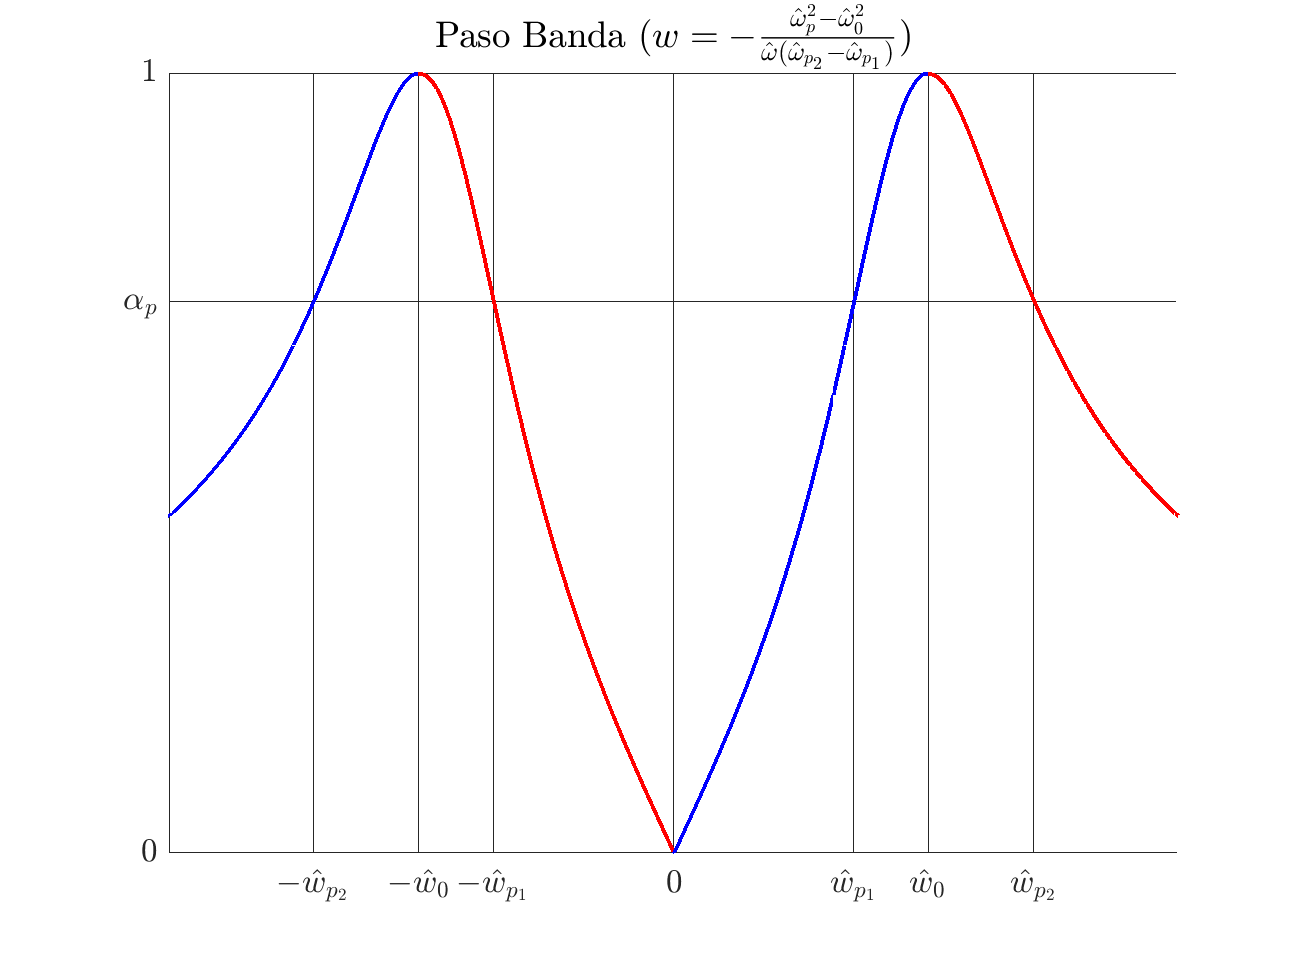
\includegraphics[height=4.25cm]{Figures/TE_2c.png}
\end{center}
\end{frame}


\begin{frame}{Transformaciones espectrales}
\begin{columns}
  \begin{column}{0.45\textwidth}
      \centering\footnotesize
      Paso bajo $\rightarrow$ Supresor de banda\\
      \[s=\omega_s\frac{\hat{s}(\hat{\omega}_{s_2}-\hat{\omega}_{s_1})}{\hat{s}^2+\hat{\omega_0}^2}\Leftrightarrow\omega=\omega_s\frac{\hat{\omega}(\hat{\omega}_{s_2}-\hat{\omega}_{s_1})}{\hat{\omega_0}^2-\hat{\omega}^2}\]\\
  \end{column}
  \begin{column}{0.55\textwidth}
      \centering
      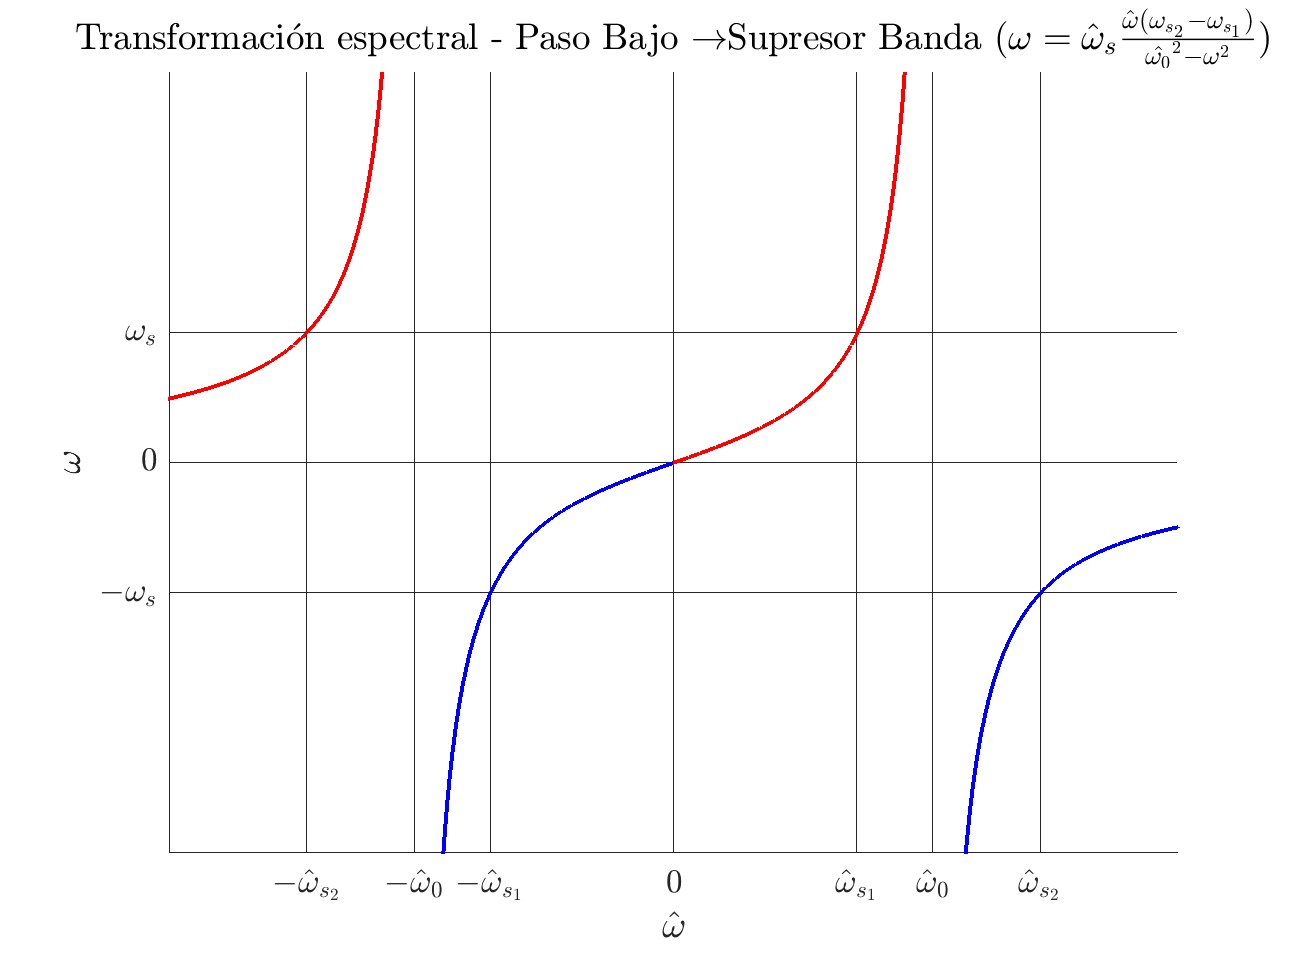
\includegraphics[height=4cm]{Figures/TE_3a.png}\\
  \end{column}
\end{columns}
\begin{center}
  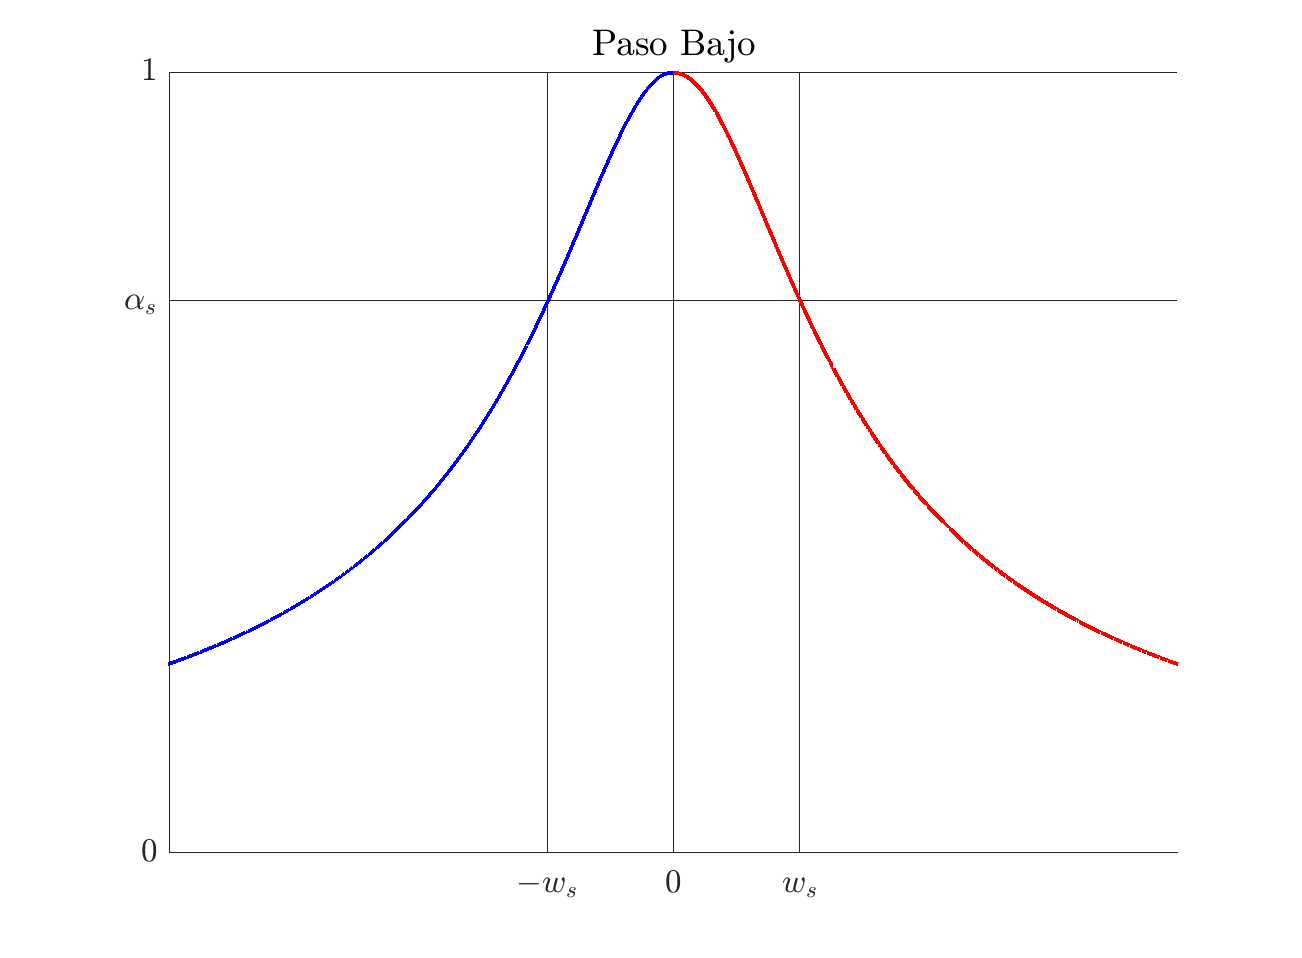
\includegraphics[height=4.25cm]{Figures/TE_3b.png}%
  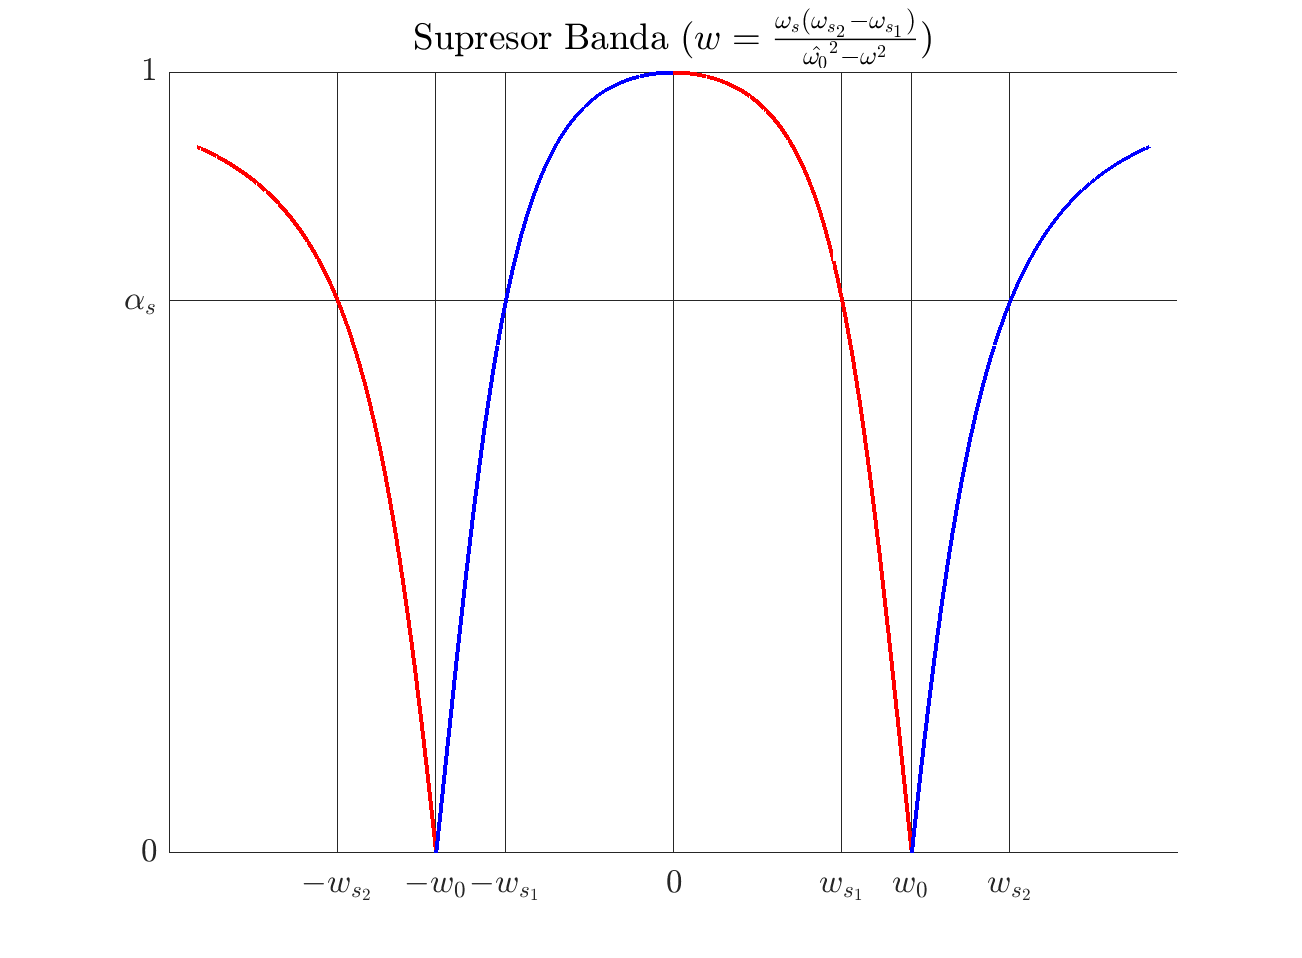
\includegraphics[height=4.25cm]{Figures/TE_3c.png}
\end{center}
\end{frame}


\begin{frame}
\frametitle{Ejemplo filtro paso alto continuo}

\footnotesize

\color{olivegreen}Diseñar un filtro de Butterworth paso altas con un borde paso banda a 4KHz, borde supresor de banda a 1KHz, rizo paso banda de 0.1dB y atenuación supresora de banda mínima 40dB.

\color{gray}
\begin{itemize}
\item $\left . \begin{array}{l}\hat \omega_p=2\pi \cdot 4000\\ \hat \omega_s=2\pi \cdot 1000\end{array}\right \}$ Suponemos $\omega_p=1 \rightarrow \omega_s=-\frac{\omega_p \hat \omega_p}{\hat \omega_s}=-4 $

\item Diseñar el filtro paso bajo con las ordenes correspondientes de Matlab

\item Convertir el filtro paso bajo a paso alta, con la relación espectral o la orden de Matlab  \alert{\texttt{[num,den]=lp2hp(num,den,$\hat{w}_p$)}}.

\end{itemize}

\begin{columns}[c]
\begin{column}{5.1cm}
\vspace{-0.5cm}
\lstinputlisting{./Matlab/ButterCode.m}
\end{column}
\begin{column}{4cm}
\vspace{0.1cm}
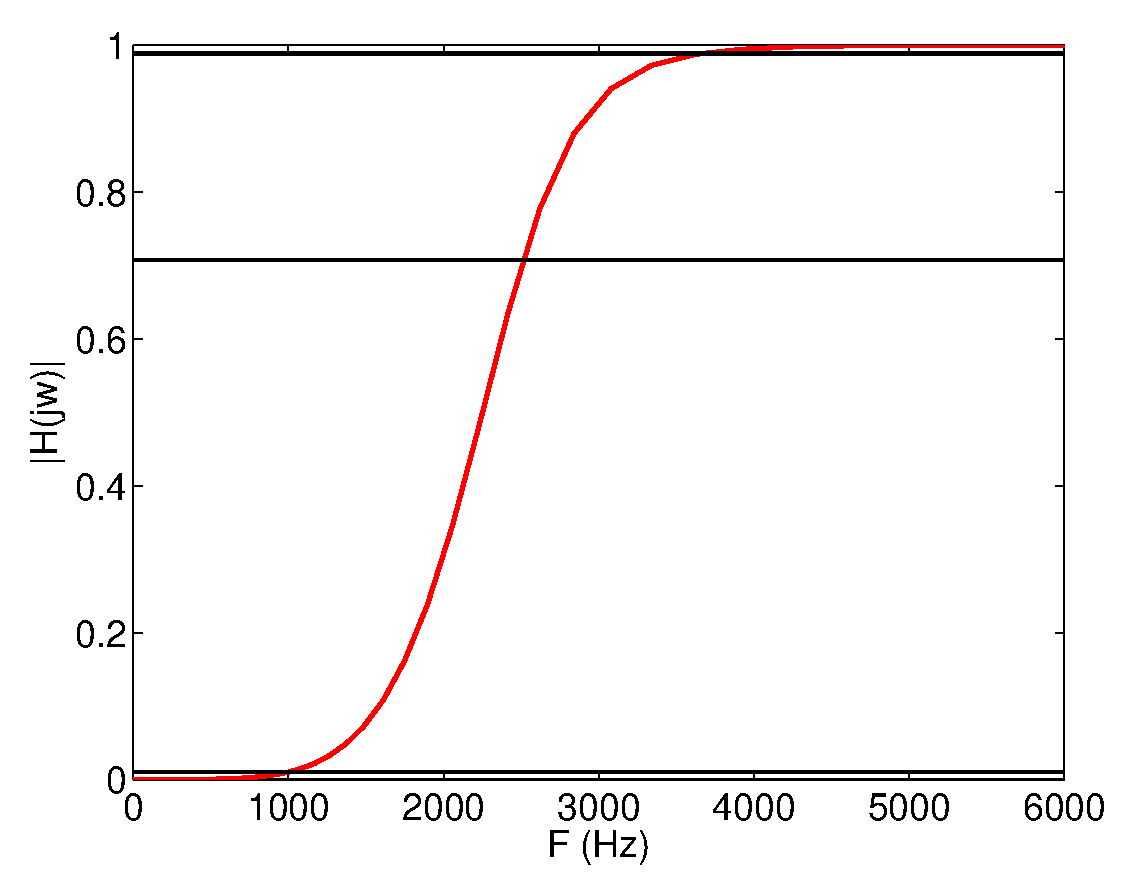
\includegraphics[width=4cm]{./Figures/FiltroButterPA.eps}
\end{column}
\end{columns}

\end{frame}


%%%%%%%%%%%%%%%%%%%%%%%%%%%%%%%%%%%%%%%%%%%%


\begin{frame}
\frametitle{Ejemplo filtro paso banda continuo}

\vspace{-0.1cm}

\footnotesize

\color{olivegreen}Diseñar un filtro elíptico con borde de la banda de paso a 4KHz y 7KHz, bordes supresores de banda a 3KHz y 8KHz, rizo de la banda de paso 1dB y atenuación superiora de banda mínima a 22dB.

\vspace{-0.1cm}

\color{gray}
\begin{itemize}

\scriptsize
\item $\left . \begin{array}{ll}\hat \omega_{p1}=2\pi \cdot 4000 & \hat \omega_{p2}=2\pi \cdot 7000\\\hat \omega_{s1}=2\pi \cdot 3000 & \hat \omega_{s2}=2\pi \cdot 8000\end{array}\right \}$ $\begin{array}{l}\omega_0^2=(2\pi)^2 \cdot 28 \cdot 10^6\\ \omega_0^2=(2\pi)^2 \cdot 24 \cdot 10^6\end{array} $



$\omega_0^2\!=\!(2\pi)^2 \!\cdot \!24 \!\cdot 10^6 \rightarrow  \hat \omega_{p1}\!=\!\frac{\omega_0^2}{\omega_{p2}}\!=\!2\pi \frac{24}{7}10^3$ $\rightarrow \hat \omega_{p2}\!-\!\hat \omega_{p1}\!=\!2\pi(7\!-\!\frac{24}{7})10^3 \!=\!2\pi \frac{25}{7}10^3 $

\vspace{-0.1cm}

Suponemos $\omega_p=1 \rightarrow \omega_s=\omega_p\frac{\hat w^2-\hat \omega_0^2}{\hat w (\hat \omega_{p2}-\hat \omega_{p1})}=\frac{9-24}{3(7-24/7)}=-1.4$

 \footnotesize

\item Diseñar el filtro paso bajo con las ordenes correspondientes de Matlab

\item Convertir el filtro paso bajo a paso alta, con la relación espectral o la orden de Matlab  \alert{\texttt{[num,den]=lp2bp(num,den,$\hat{w}_0$,$\hat{w}_{p2}-\hat \omega_{p1}$)}}.

\end{itemize}

\vspace{-0.1cm}

\begin{columns}[c]
\begin{column}{5.1cm}
\vspace{-0.5cm}
\lstinputlisting{./Matlab/EllipCode.m}
\end{column}
\begin{column}{4cm}
\vspace{0.1cm}
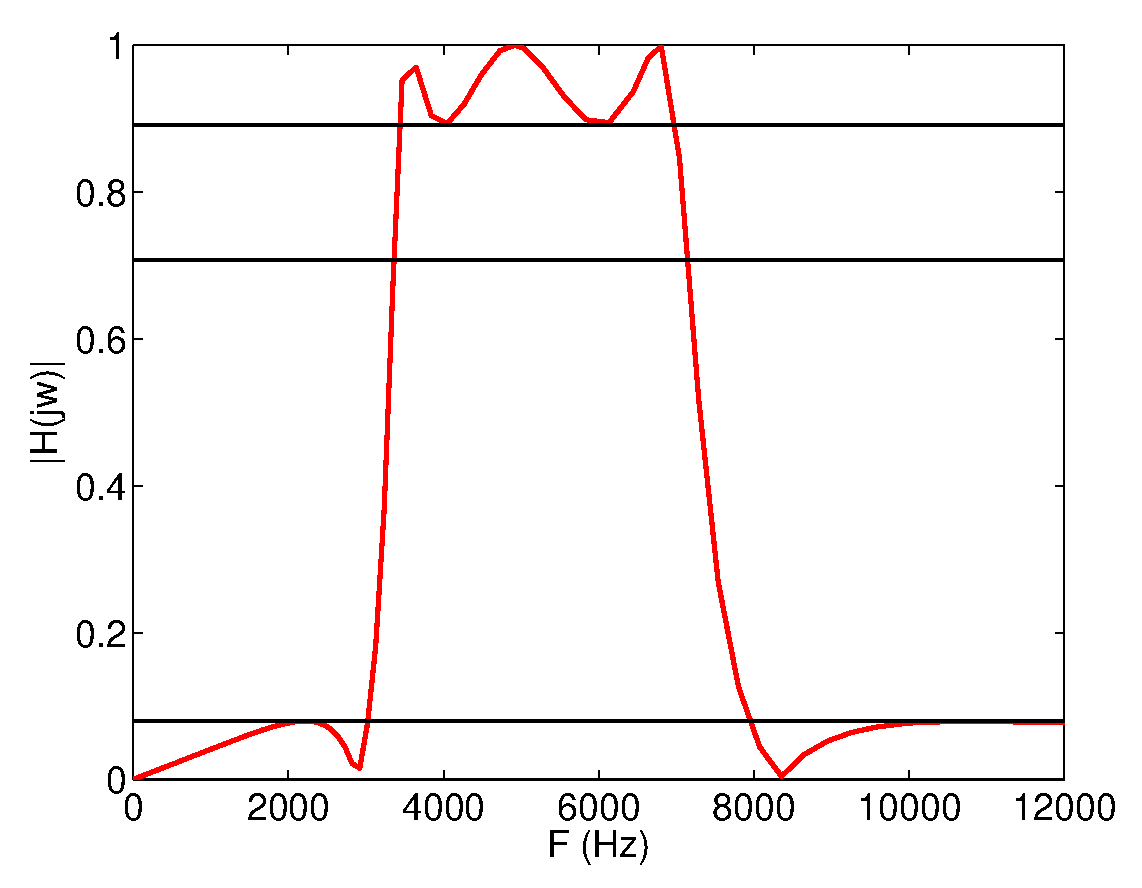
\includegraphics[width=4cm]{./Figures/FiltroEllipPB.eps}
\end{column}
\end{columns}

\end{frame}


%%%%%%%%%%%%%%%%%%%%%%%%%%%%%%%%%%%%%%%%%%%%

\begin{frame}
\frametitle{Ejemplo filtro supresor de banda continuo}

\vspace{-0.1cm}

\footnotesize

\color{olivegreen}Diseñar un filtro de Chebyshev tipo II con borde de la banda de paso a 4KHz y 7KHz, bordes supresores de banda a 5KHz y 6KHz, rizo de la banda de paso 2dB y atenuación superiora de banda mínima a 30dB.

\vspace{-0.1cm}

\color{gray}
\begin{itemize}

\scriptsize
\item $\left . \begin{array}{ll}\hat \omega_{p1}=2\pi \cdot 4000 & \hat \omega_{p2}=2\pi \cdot 7000\\\hat \omega_{s1}=2\pi \cdot 5000 & \hat \omega_{s2}=2\pi \cdot 6000\end{array}\right \}$ $\begin{array}{l}\omega_0^2=(2\pi)^2 \cdot 28 \cdot 10^6\\ \omega_0^2=(2\pi)^2 \cdot 30 \cdot 10^6\end{array} $



$\omega_0^2\!=\!(2\pi)^2 \!\cdot \!28 \!\cdot 10^6 \rightarrow  \hat \omega_{s1}\!=\!\frac{\omega_0^2}{\omega_{s2}}\!=\!2\pi \frac{28}{6}10^3$ $\rightarrow \hat \omega_{s2}\!-\!\hat \omega_{s1}\!=\!2\pi(6\!-\!\frac{28}{6})10^3 \!=\!2\pi \frac{8}{6}10^3 $

\vspace{-0.1cm}

Suponemos $\omega_s=1 \rightarrow \omega_p=\omega_s\frac{\hat \omega_p (\hat \omega_{s2}-\hat \omega_{s1})}{\hat \omega_0^2-\hat \omega_p^2}=\frac{4(6-28/6)}{28-16}=0.44$

 \footnotesize

\item Diseñar el filtro paso bajo con las ordenes correspondientes de Matlab

\item Convertir el filtro paso bajo a paso alta, con la relación espectral o la orden de Matlab  \alert{\texttt{[num,den]=lp2bs(num,den,$\hat{w}_0$,$\hat{w}_{s2}-\hat \omega_{s1}$)}}.

\end{itemize}

\vspace{-0.1cm}

\begin{columns}[c]
\begin{column}{5.1cm}
\vspace{-0.5cm}
\lstinputlisting{./Matlab/ChebyCode.m}
\end{column}
\begin{column}{4cm}
\vspace{0.1cm}
\includegraphics[width=4cm]{./Figures/FiltroChebySB1.eps}
\end{column}
\end{columns}

\end{frame}


%%%%%%%%%%%%%%%%%%%%%%%%%%%%%%%%%%%%%%%%%%%%


\begin{frame}
\frametitle{Filtro continuos con Matlab}

\footnotesize
\begin{itemize}
\item Alternativamente se puede hacer todo en un único paso con las funciones de Matlab que ya conocemos.
\item Veamos un ejemplo con las de Chebyshev de tipo II
\begin{itemize}
\item \alert{\texttt{[N,wn]=cheb2ord(wp,ws,alphap,alphas,'s');}}

\vspace{0.1cm}

{\footnotesize
\hspace{0.5cm}Paso bajo: wp=3, ws=5;

\vspace{0.1cm}

\hspace{0.5cm}Paso alto: wp=5, ws=3;

\vspace{0.1cm}

\hspace{0.5cm}Paso banda: wp=[5 7], ws=[4 8];

\vspace{0.1cm}

\hspace{0.5cm}Eliminación de banda: wp=[5 7], ws=[5.5 6.5];}

\vspace{0.1cm}

\item\alert{\texttt{[num,den]=cheby2(N,alphas,wn,tipo,'s');}}

\vspace{0.1cm}

\hspace{0.5cm}tipo: 'low', 'high', nada, 'stop'
\end{itemize}

\end{itemize}

\end{frame}

%%%%%%%%%%%%%%%%%%%%%%%%%%%%



\begin{frame}
\frametitle{Ejemplos de filtros continuos con Matlab I}

\vspace{-0.1cm}

\footnotesize

\color{olivegreen}Diseñar un filtro de Butterworth paso altas con un borde paso banda a 4KHz, borde supresor de banda a 1KHz, rizo baso banda de 0.1dB y atenuación supresora de banda mínima 40dB.

\vspace{-0.15cm}

\color{gray}

\begin{columns}[c]
\begin{column}{6cm}
\vspace{-0.5cm}
\lstinputlisting{./Matlab/ButterCode2.m}
\end{column}
\begin{column}{4cm}
\vspace{0.1cm}
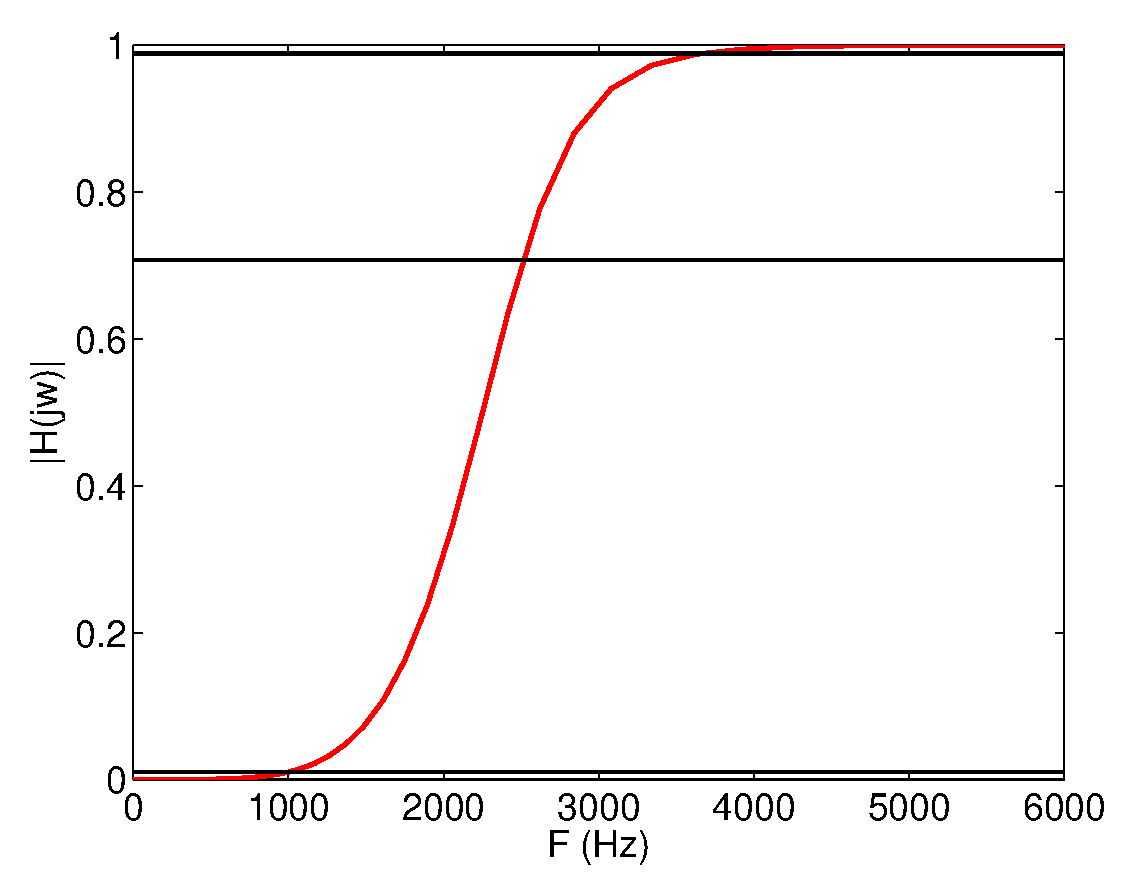
\includegraphics[width=3.8cm]{./Figures/FiltroButterPA.eps}
\end{column}
\end{columns}

\vspace{-0.15cm}

\color{olivegreen}Diseñar un filtro elíptico con borde de la banda de paso a 4KHz y 7KHz, bordes supresores de banda a 3KHz y 8KHz, rizo de la banda de paso 1dB y atenuación superiora de banda mínima a 22dB.

\vspace{-0.1cm}

\color{gray}

\begin{columns}[c]
\begin{column}{6cm}
\vspace{-0.5cm}
\lstinputlisting{./Matlab/EllipCode2.m}
\end{column}
\begin{column}{4cm}
\vspace{0.1cm}
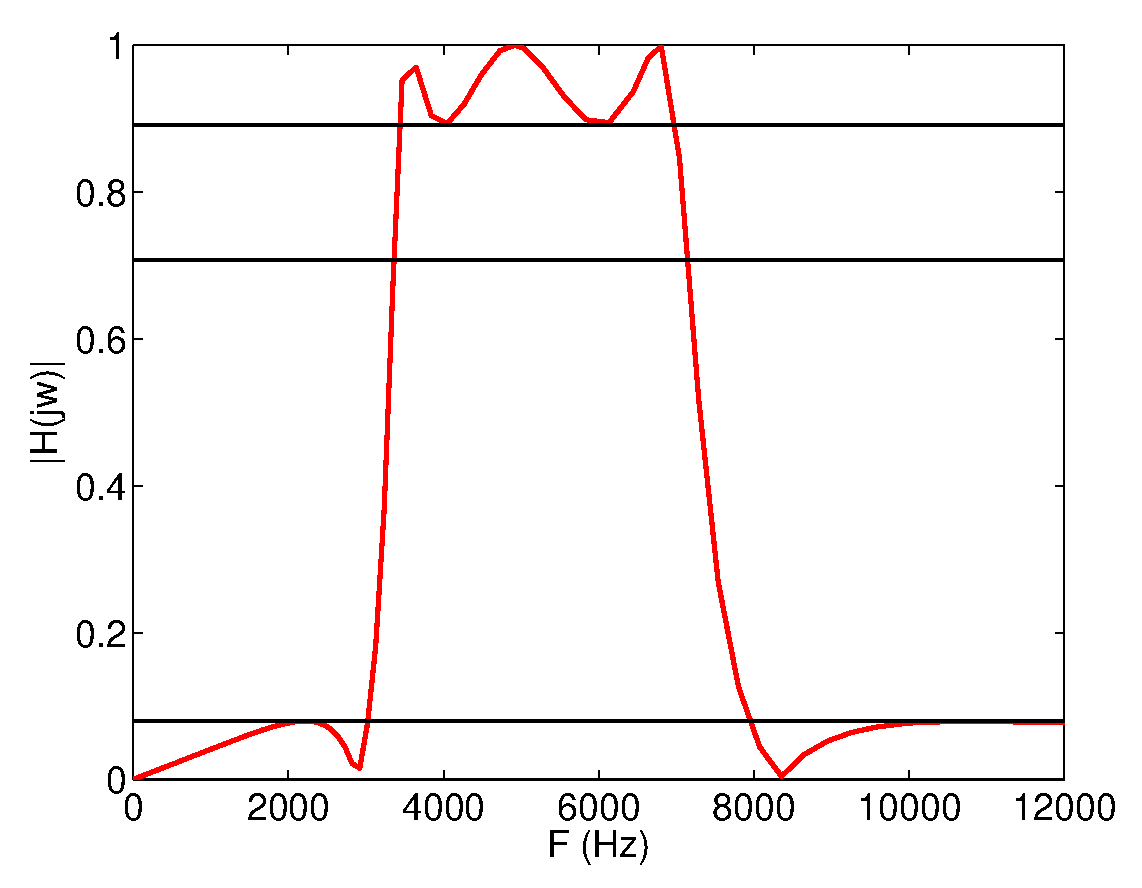
\includegraphics[width=3.8cm]{./Figures/FiltroEllipPB.eps}
\end{column}
\end{columns}

\end{frame}

%%%%%%%%%%%%%%%%%%%%%%%%%%%%%%%%%%%%%%%%%%%%%%%%


\begin{frame}
\frametitle{Ejemplos de filtros continuos con Matlab II}

\vspace{-0.1cm}

\footnotesize

\color{olivegreen}Diseñar un filtro de Chebyshev tipo I supresor de banda con borde de la banda supresora de 2 KHz a 6 KHz, borde de la banda de paso de 1KHz a 7 KHz, rizo baso banda de 0.5dB y atenuación supresora de banda mínima 20dB.

\vspace{0.2cm}


\color{gray}

\begin{columns}[c]
\begin{column}{6cm}
\vspace{-0.5cm}
\lstinputlisting{./Matlab/ChebyCode2.m}
\end{column}
\begin{column}{4cm}
\vspace{0.1cm}
\includegraphics[width=3.8cm]{./Figures/FiltroChebySB.eps}
\end{column}
\end{columns}

\vspace{-0.15cm}



\end{frame}

%%%%%%%%%%%%%%%%%%%%%%%%%%%%%%%%%%%%%%%%%%%%%%%%
